\documentclass{article}

\usepackage{arxiv}

\usepackage{threeparttable}
\usepackage{tabularx}
\usepackage{arydshln}
\usepackage{booktabs}
\usepackage{times}
\usepackage{epsfig}
\usepackage{graphicx}
\usepackage{amsmath}
\usepackage{amssymb}
\usepackage[english]{babel}
\usepackage{pdfrender}
\newcommand*{\boldcheckmark}{%
  \textpdfrender{
    TextRenderingMode=FillStroke,
    LineWidth=.5pt, % half of the line width is outside the normal glyph
  }{\checkmark}%
}
\usepackage{hyperref}
\usepackage{url}
\usepackage{cleveref}
\hypersetup{colorlinks}
\usepackage{mathtools}
\usepackage{dpr}
\usepackage{fec}
\usepackage{enumerate}
\usepackage{subcaption}
\usepackage{algorithm,algpseudocode}
\usepackage{makecell}
\usepackage{comment}
\usepackage{caption}
\usepackage{subcaption}
\usepackage{enumitem}
\usepackage{amsthm}
\usepackage{bm}
\usepackage{siunitx,tabularx,ragged2e} % ,booktabs
\usepackage{wrapfig}
\usepackage{float}
\usepackage{pifont}
\usepackage{soul}
\usepackage{epstopdf}
\usepackage{blindtext}
\usepackage{fancyvrb}
\usepackage{multirow, booktabs}
\usepackage{cleveref}
\usepackage{hhline}
\usepackage{textcomp}
\usepackage{tcolorbox}
\usepackage{MnSymbol}
\usepackage{amssymb,fge}
\usepackage{setspace}
\usepackage{subcaption}
\usepackage{bbding}
\usepackage{cleveref}
\usepackage{hhline}
%Import the natbib package and sets a bibliography  and citation styles
\usepackage{natbib}
\bibliographystyle{abbrvnat}
\setcitestyle{authoryear,open={(},close={)}} %Citation-related commands


\definecolor{darkpastelgreen}{rgb}{0.01, 0.75, 0.24}
\definecolor{electriccrimson}{rgb}{1.0, 0.0, 0.25}
\definecolor{navyblue}{rgb}{0.0, 0.0, 0.75}
\newcommand{\ie}{\textit{i.e.}}
\newcommand{\eg}{\textit{e.g.}}
% \newcommand{\tc}[1]{{\color{blue}#1}}
% \newcommand{\dz}[1]{{\color{electriccrimson}DZ: #1}}
% \newcommand{\dzc}[1]{\colorbox{yellow}{\color{electriccrimson}DZ: #1}}
% \newcommand{\csh}[1]{{\color{navyblue}SC: #1}}
% \newcommand{\jk}[1]{{\color{darkpastelgreen}JK: #1}}

\theoremstyle{plain}
\newtheorem{theorem}{Theorem}[section]
\newtheorem{proposition}[theorem]{Proposition}
\newtheorem{lemma}[theorem]{Lemma}
\newtheorem{corollary}[theorem]{Corollary}
\theoremstyle{definition}
\newtheorem{definition}[theorem]{Definition}
\newtheorem{assumption}[theorem]{Assumption}
\newtheorem{remark}[theorem]{Remark}

\newcommand{\algacro}{WINA{}}

\newcommand{\ycell}[1]{\colorbox{yellow!60}{\strut #1}}

\newcommand{\cmark}{\textcolor{green!70!black}{\small\ding{51}}}
\newcommand{\xmark}{\textcolor{red}{\small\ding{55}}}

\title{\algacro{}: Weight Informed Neuron Activation for Accelerating Large Language Model Inference}


\author{
Sihan Chen$^{2\ddagger}$\thanks{Primary author, \texttt{\url{chensihan@ruc.edu.cn}}.}\ \ \ Dan Zhao$^{3\S}$\ Jongwoo Ko$^{1}$\ \  Colby Banbury$^{1}$\ \  Huiping Zhuang$^{4}$\ \  Luming Liang$^{1}$\ \  Tianyi Chen$^{1\ddagger}$\thanks{Corresponding author, \texttt{\url{Tianyi.Chen@microsoft.com}}.}\\
$^1$Microsoft\quad $^2$Renmin University of China\quad $^3$New York University\quad $^4$South China University of Technology\\
$\ddagger$Equal contributions.\quad $\S$ Work is done at Microsoft.
}

\begin{document}

\maketitle

\begin{abstract}
The growing computational demands of large language models (LLMs) make efficient inference and activation strategies increasingly critical. While recent approaches, such as Mixture-of-Experts (MoE), leverage selective activation but require specialized training, training-free sparse activation methods offer broader applicability and superior resource efficiency through their plug-and-play design. However, many existing methods rely solely on hidden state magnitudes to determine activation,  resulting in high approximation errors and suboptimal inference accuracy. To address these limitations, we propose \textbf{\algacro{}} (\textbf{W}eight \textbf{I}nformed \textbf{N}euron \textbf{A}ctivation), a novel, simple, and training-free sparse activation framework that jointly considers hidden state magnitudes and the column-wise $\ell_2$-norms of weight matrices. We show that this leads to a sparsification strategy that obtains optimal approximation error bounds with theoretical guarantees tighter than existing techniques. Empirically, \algacro{} also outperforms state-of-the-art methods (\eg, TEAL) by up to 2.94\% in average performance at the same sparsity levels, across a diverse set of LLM architectures and datasets. These results position \algacro{} as a new performance frontier for training-free sparse activation in LLM inference, advancing training-free sparse activation methods and setting a robust baseline for efficient inference. The source code is available at \url{https://github.com/microsoft/wina}.
\end{abstract}

\section{Introduction}

While large language models (LLMs) have revolutionized the field of natural language processing, offering unprecedented capabilities in a variety of applications, such as text generation~\citep{li2024pre,cheng2025dehumanizing}, translation~\citep{hendy2023goodgptmodelsmachine,seamless2025joint},  understanding~\citep{chang2024survey,tschannen2025siglip}, and grounding~\citep{zhao2025robustness,hui2025winclick} their growing size and complexity make controlling their computation costs challenging. They often require substantial computational resources, particularly during inference, making reducing inference costs without degrading output quality a central challenge.

One strategy has been to activate only a sub-network of the full model~\citep{jacobs1991adaptive} during inference using a Mixture of Experts (MoE) architecture, which has already seen adoption in popular and widely-used LLMs like GPT4~\citep{achiam2023gpt} and Mistral~\citep{jiang2023mistral}. Other methods include model distillation, where a smaller model is trained using knowledge distilled from a larger teacher model to route inference requests more efficiently. However, these approaches can require a considerable amount of training, which can also be computationally costly.

An alternative is training-free sparse activation, which retains the original dense model but selectively omits weights or neurons at inference time. These training-free methods avoid training or retraining and can be applied to off-the-shelf models. They leverage criteria such as hidden-state magnitudes, weight importance, weight statistics, or additional validation data to determine which parts of the model to deactivate, thereby accelerating inference.
% To tackle these challenges, the Mixture of Experts (MoE) activates only a sub-network during inference, thereby economizing computational cost~\citep{jacobs1991adaptive}. MoE offers a promising solution and has been successfully employed in commercial LLMs such as GPT4~\citep{achiam2023gpt} and Mistral~\citep{jiang2023mistral}.}
% }



% \csh{
However, current training-free methods exhibit critical limitations. Most notably, they ignore the influence of weight matrices on error propagation. Specifically, these approaches fail to account for how interactions between input elements and the weight matrix during forward propagation affect model outputs, leading to accumulated approximation errors in sparse activation.

\paragraph{Contributions.} In this paper, we propose \algacro{}: a simple, easy-to-use, training-free framework that performs sparse activation based on the magnitude of hidden states and the column-wise $\ell_2$-norm of the weight matrix. By combining activation strength with weight importance, our thresholds directly reflect how much each activation can influence the next layer. This design provides theoretical guarantees that the total approximation error remains bounded and is lower than that of other comparable approaches. 

In contrast, methods like TEAL rely exclusively on the distribution of hidden‐state magnitudes to decide which activations to keep and which to deactivate. Ignoring weight magnitudes in this way may discard highly influential activations or retain many low‐impact ones, leading to suboptimal trade-offs between efficiency and output quality. Our framework overcomes these limitations by integrating weight statistics into the selection process, achieving finer control over sparsity and tighter bounds on the resulting approximation error.

% By ranking columns according to this bound and pruning those with smallest contributions, \algacro{} ensures that the total approximation error remains below a user-defined threshold, and we provide a theoretical proof of this guarantee.

\begin{wraptable}{r}{0.42\textwidth}
\centering
\scriptsize
% \resizebox{1.0\columnwidth}{!}{
	\vspace{-3.5mm}
	\begin{tabular}{lccc}
		\toprule
		& \textbf{\algacro{}} & \textbf{TEAL}  & \textbf{CATS}  \\
		\midrule
		\textbf{Tight Approx Error}  & {\cmark} & \xmark & \xmark \\
		\textbf{Layer Generality} & \cmark & \cmark & \xmark  \\
		\textbf{Hetero Sparsity} & \cmark & \cmark & \xmark  \\
		\bottomrule
	\end{tabular}
	\vspace{-3mm}
\end{wraptable}
We evaluate \algacro{} on multiple widely-used LLMs (ranging from 7B to 14B parameters) across several popular benchmark datasets. Compared with state-of-the-art training-free methods such as TEAL~\citep{liu2024trainingfreeactivationsparsitylarge} and CATS~\citep{lee2024catscontextuallyawarethresholdingsparsity}, achieves superior model performance at identical sparsity levels, with significantly less performance degradation. 
We also establish theoretical error bounds for our methodology,  providing formal support for the experimental results and validating our method's effectiveness. In summary, our detailed contributions include as follows.


\begin{itemize}[leftmargin=*, itemsep=3pt]
	\item \textbf{Weighted-informed Activation:} we introduce a novel sparse activation method that jointly considers hidden state magnitudes and the column-wise $\ell_2$-norms of weight matrices. This allows for selecting neurons that are not only strongly activated but also those that have a larger influence on downstream layers, leading to a more informed construction of a sub-network during inference.
	\item \textbf{Theoretically Tighter Approximation Error:} {we conduct a formal analysis to demonstrate that our weight-informed activation mechanism yields a lower expected output error compared to prior methods (e.g., TEAL) under mild assumptions, including column-wise orthogonality of weights and monotonic activation functions, with guarantees extendable to multi-layer architectures.}
	\item \textbf{Numerical Experiments:} {we perform extensive evaluations on multiple LLMs, including Qwen-2.5 \citep{bai2023qwen}, LLaMA series~\citep{touvron2023llama}, and Phi-4~\citep{abdin2024phi}, demonstrate that our method achieves superior accuracy under various sparsity levels. In particular, \algacro{} maintains better performance as sparsity increases, highlighting its robustness and practical utility across diverse tasks and model scales.}
\end{itemize}

The rest of our paper is organized as follows. We begin by reviewing related works in Section \ref{sec:related_work}. We detail our methodology in Section \ref{sec:algo} and review our experimental results in Section \ref{sec:experiments}. We conclude with a discussion on future directions in Section \ref{sec:conclusion}.

% \begin{table}[h]
	% \centering
	% \renewcommand{\arraystretch}{1.3}
	% \setlength{\tabcolsep}{6pt}
	% \begin{tabular}{lccc}
		% \toprule
		%  & \textbf{CATS} & \textbf{TEAL} & \textbf{WINA} \\
		% \midrule
		% Sparsity for all matrices & \XSolidBrush & {\textcolor{Green}{\CheckmarkBold}} & \CheckmarkBold \\
		% Different sparsity for each matrix   & \XSolidBrush & \CheckmarkBold      & \CheckmarkBold\\
		% Error control & \XSolidBrush & \XSolidBrush & \CheckmarkBold \\
		% \bottomrule
		% \end{tabular}
	% \end{table}


\section{Related Work}
\label{sec:related_work}

\paragraph{Sparse Activation.} Modern sparse activation activation approaches fall into two principal paradigms: training-based methods and training-free methods. Training-based methods typically employ a trainable router to learn to dynamically select activated experts for each token, with the Mixture-of-Experts (MoE) architecture~\citep{jacobs1991adaptive} serving as the foundational framework. In this framework, each expert operates an individual component of the model, as only the relevant experts are activated for each input during inference, achieving significant computational savings.

This paradigm has been expanded through many iterations and variants. The sparsely-gated mixture of experts layer \citep{shazeer2017outrageously} integrates MoE into recurring neural networks (RNNs). Works like GShard \citep{lepikhin2020GShard} and the Switch Transformer \citep{fedus2022switch} extend MoEs to the Transformer architecture \citep{raffel2020exploring} while others combine several approaches, such as WideNet~\citep{xue2022go},  reduces the size of the MoE model by initially compressing the model before transitioning into a MoE. Works like MoEBert \citep{zuo2022moebert} decomposes the FFN layer of a pre-trained dense model into multiple experts based on importance-guided adaptation and then refines the model through distillation. LLM in Flash \citep{alizadeh2023llm} employs a low-rank predictor to determine which intermediate neurons are activated.

Training-free methods, in contrast, do not rely on a learnable router, instead using predefined or calculated criteria to perform sparse activation. Methods \citep{han2015learnweightsconnect} can utilize magnitude-based weight pruning or global activation pruning \citep{wen2016learnstructsparse} to apply a fixed sparsity pattern regardless of input. For instance, Q-Sparse \citep{wang2024q} produces sparsity as a function of input magnitudes, achieving sparsity rates of 60\% with reasonable performance degradation. CATS~\citep{lee2024catscontextuallyawarethresholdingsparsity} applies sparse activation on SwiGLU outputs within gated MLP layers, achieving performance comparable to the original dense model while achieving  25\% model sparsity. In contrast, TEAL~\citep{liu2024trainingfreeactivationsparsitylarge} extends magnitude-based activation sparsity to all network layers, achieving 40-50\% model-wide sparsity across architectures with minimal performance impact. 

However, current sparse activation methods suffer from noticeable limitations. They determine activation elements solely based on the magnitude of hidden states, neglecting the crucial influence of the weight matrix, which results in suboptimal error control.

\paragraph{Relations to Model Structured Pruning.} Although \algacro{} shares the shared goal of reducing inference cost with structured pruning methods (via a similar paradigm by searching a sub-network), its philosophy and mechanism differ substantially. Traditional model pruning removes redundant parameters from deep neural networks~\citep{han2015deep, frankle2018lottery, frantar2023sparsegpt}, often requiring fine-tuning to restore performance~\citep{lin2019toward, he2018soft, wen2016learning, li2020group, zhuang2020neuron, chen2017reduced, chen2021orthant, chen2020neural}. To enhance the quality of the pruned sub-networks, recent advances introduce knowledge-transfer mechanisms during pruning~\citep{chen2021oto, chen2023otov2, chen2023otov3, chen2023lorashear, chen2024hesso,qu2025automatic} or apply post-hoc distillation~\citep{ko2024distillm, ko2025distillm} to improve accuracy. However, these approaches typically involve additional training stages, making them less suitable for scaling to large foundation models. In contrast, \algacro{} is a training-free, plug-and-play sparse activation framework that dynamically selects high-performing sub-networks at inference time without modifying or retraining the model. This makes \algacro{} particularly well-suited for deployment in resource-constrained or latency-sensitive environments.


% \textbf{Model Pruning}.
% Unstructured pruning \citep{frankle2018lottery, sanh2020movement}, which targets individual neurons rather than structured blocks, often yields higher compression rates but is generally not conducive to model speedup improvements. While structured pruning has emerged as a critical model compression technique, particularly in the domain of large language model~\citep{kurtic2024ziplm, ma2023llm} for its ability to accelerate model inference and address the challenges posed by the ever-growing model sizes with minimal impact on performance. 

% Structured pruning approaches can be divided into either multi-stage or end-to-end. Multi-stage pruning \citep{xia2023sheared, frantar2023sparsegpt} involves an initial phase where fully-trained models are analyzed to identify and eliminate redundant structures to construct a slimmer DNN. Subsequently, the pruned model may undergo retraining to recover any loss in accuracy, potentially employing knowledge distillation techniques. This method is complex and time-intensive, necessitating multiple training iterations of DNN and substantial domain knowledge to manually proceed each step effectively. End-to-end pruning amis to avoid fine-tuning by enabling training once to compress the model. Advances such as OTOv2 \citep{chen2023otov2} and DepGraph \citep{fang2023depgraph} have further automated the structured pruning process for general DNNs, reducing the manual efforts required to discern removal structures and construct a slimmer model. OTOv3 \citep{chen2023otov3} extends the pruning mode to a new application domain to automatically erase redundant operators entirely, enabling the automatic and generic of structured pruning.

% \dz{
% \paragraph{Expansion \& Upcycling.} 
% In attempts to more easily realize the efficiency gains of MoE architectures for LLMs, more recent work has focused on upcycling: the process of converting a trained dense model into a MoE model. 
% Recent work \cite{upcycle} has created large-scale MoE from LLMs as existing pre-trained
% checkpoints, which has already seen usage and adoption among popular language models \cite{deepseeek2024, bai2023qwen}. 
% }

% \begin{table}[!ht]
%     \centering
%     \caption{Summary of \algacro{} and existing methods}
%     \resizebox{1.0\linewidth}{!}{
%     \begin{tabular}{l|lll}
%     \toprule[0.1em]
%         \textbf{} & \textbf{Additional model size} & \textbf{Efficient Routing} & \textbf{Generic} \\ 
%         \midrule
%         Classial MoE & large & No & No \\ 
%         In-place MoE & little & No & No \\ 
%         \algacro{} & little & Yes & Yes \\ 
%         \bottomrule[0.1em]
%     \end{tabular}
%     }
% \end{table}
% \section{Algorithm}
\section{Methodology}
\label{sec:algo}

{
	We now present \algacro{}, a framework for sparse activation that preserves critical elements while zeroing out non-essential components in each layer's input. As illustrated in Figure~\ref{fig:Overview}, \algacro{} jointly considers both the input tensor and the associated weight matrix, rather than relying solely on input magnitudes. During inference, it activates only the most influential neurons, effectively constructing a sparse sub-network that maintains the expressive power of the original model.
}

\begin{figure}
	\centering
	% \includegraphics[width=\textwidth]{figures/Overview.png}
	% \includegraphics[width=0.8\textwidth]{figures/adaloro_algo_fig.pdf}
	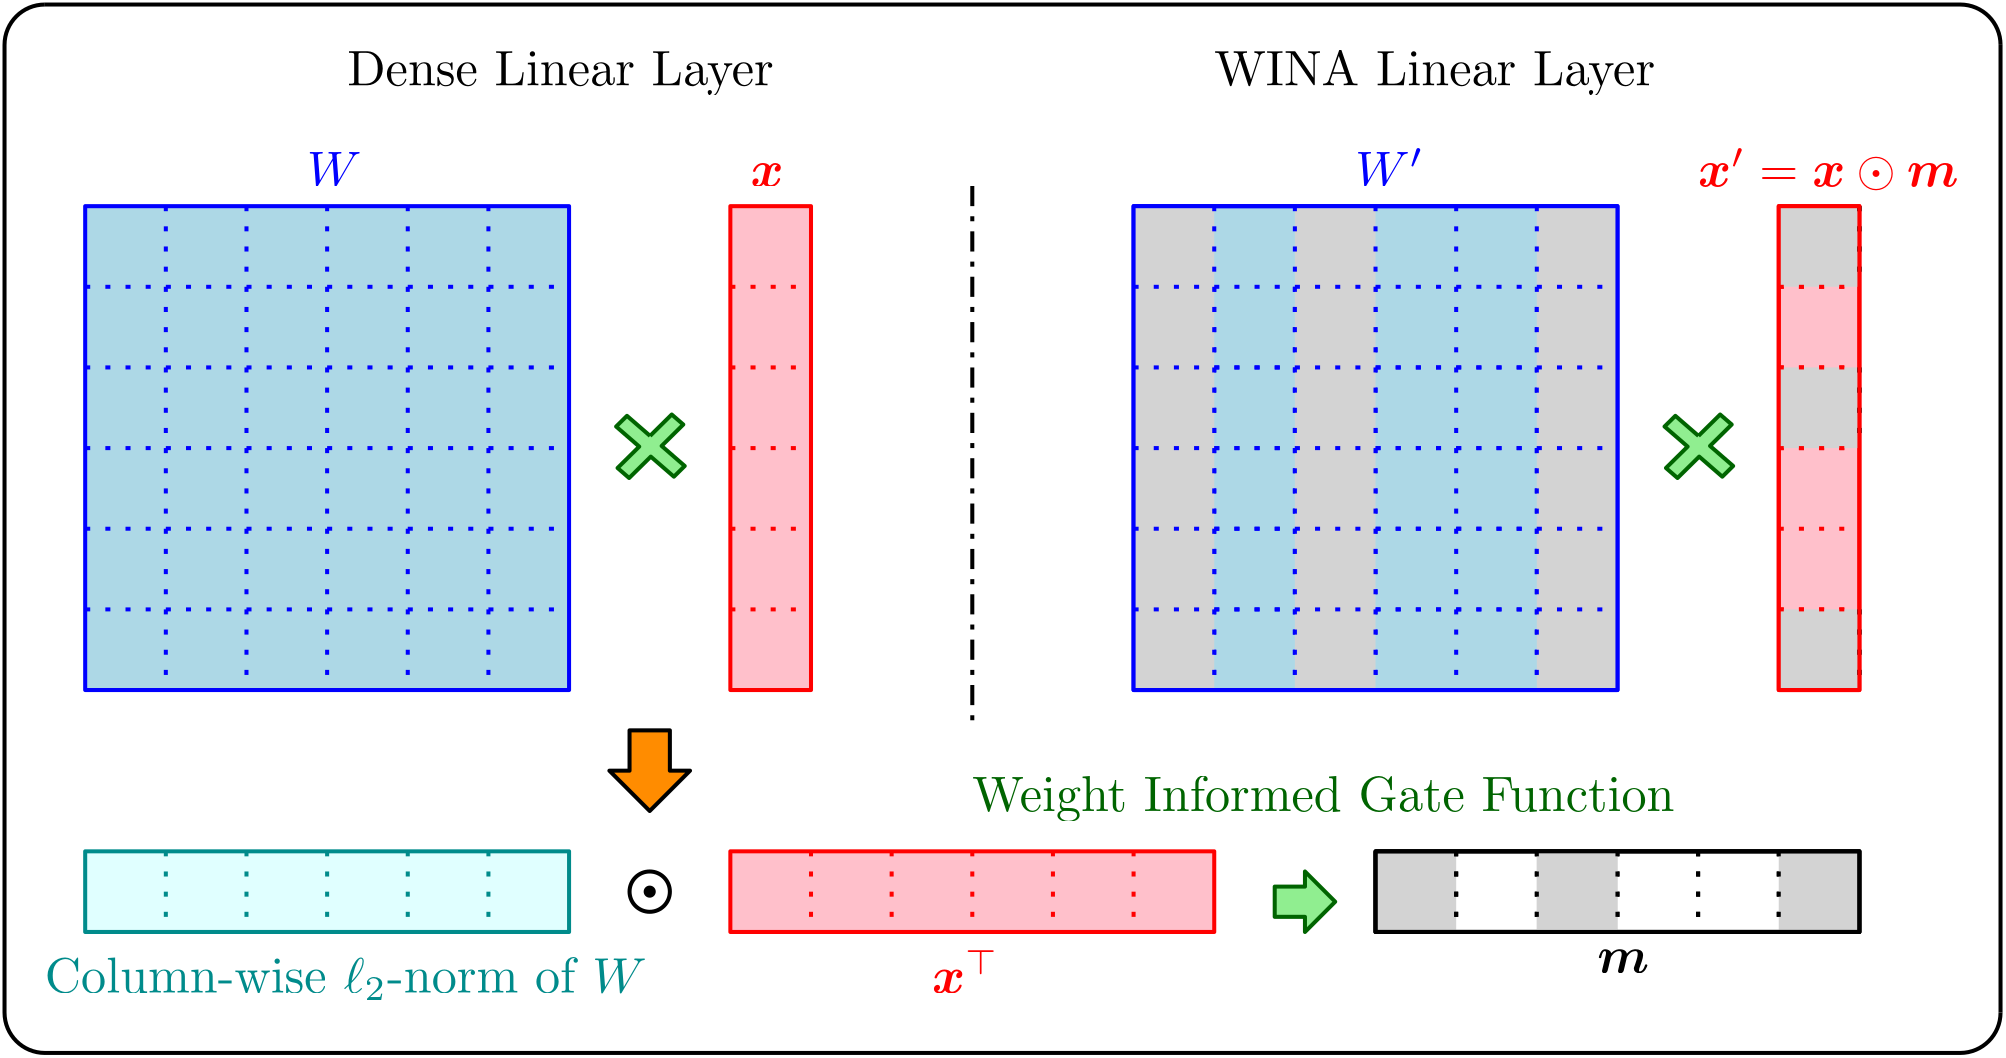
\includegraphics[width=0.8\textwidth]{overview.png}
	\caption{{\textbf{Overview of \algacro{}.} \algacro{} performs training-free sparse activation by selecting the most influential input dimensions based on both hidden state magnitudes and the column-wise $\ell_2$-norms of weight matrices. This joint criterion ensures accurate sub-network activation at each layer during inference, preserving model performance while reducing computational overhead.}}
	\label{fig:Overview}
\end{figure}

\subsection{Problem Statement}

{
	\textbf{Main Problem.}  
	Consider a deep neural network (DNN) $\mathcal{M}$ consisting of $L$ layers. We denote the weight matrix of the $l$-th layer as $W_l \in \mathbb{R}^{m_l \times n_l}$ and the corresponding input as an arbitrary tensor $X \in \mathbb{R}^{n_l \times s_l}$ for $l \in \{1, ..., L\}$, representing the full information content.  
	Our goal is to identify a set of binary activation gates $\mathcal{G} = \{\bm{g}_1, \cdots, \bm{g}_L\}$, where each $\bm{g}_l \in \{0, 1\}^{n_l}$, such that the deviation between the model's original output and the gated output is minimized:
	\begin{equation}
		\mathop{\text{minimize}}_{\bm{g}_1, \cdots, \bm{g}_L} \quad \norm{\mathcal{M}(X) - \mathcal{M}(X \mid \mathcal{G})}_2.
	\end{equation}
	
	Since obtaining the complete set of possible inputs $X$ is generally infeasible, we instead use a sampled subset $\tilde{X}$ to approximate it. The activation gating operates in the input vector space to reduce output deviation. With this observation, we can reformulate the original problem into a per-layer version to make the problem more tractable.
	
	\textbf{Refined Problem.}  
	Given a weight matrix $W \in \mathbb{R}^{m \times n}$ and a sampled input vector $\bm{x} \in \mathbb{R}^{n}$, the standard linear transformation is $\bm{y} \gets W \bm{x}$.  
	Our objective then becomes identifying an activation gate or mask $\bm{m} \in \{0, 1\}^{n}$ such that the masked output $\bm{y}_{\bm{m}} \gets W(\bm{m} \odot \bm{x})$ approximates the original by solving:
	\begin{equation}\label{main.prob}
		\mathop{\text{minimize}}_{\bm{m} \in \{0, 1\}^{n}} \quad  \norm{W \bm{x} - W(\bm{m} \odot \bm{x})}_2.
	\end{equation}
}

\subsection{Weight Informed Gate Function}

\textbf{Motivation.}
Many current sparse activation methods (\eg, Q-sparse~\citep{wang2024q}, CATS~\citep{lee2024catscontextuallyawarethresholdingsparsity}, TEAL~\citep{liu2024trainingfreeactivationsparsitylarge}) operate via a top-$K$ gating mechanism governed by the absolute values of the hidden states:
\begin{equation}
	\bm{m}_i = \begin{cases}
		1 & \text{if } |\bm{x}_i| \text{ is among the top-$K$ values in } |\bm{x}|, \\
		0 & \text{otherwise}
	\end{cases}
\end{equation}
However, this approach ignores the critical role that weight matrices play. Specifically, how each element of the preceding input interacts with the weight matrix $W$ in the forward propagation. This mismatch motivates us to propose \algacro{}, a method that jointly considers both inputs and weight matrices to minimize the approximation error for better performance.

\textbf{Formalization.}
In \algacro{}, we construct binary activation gates by selecting the top-$K$ components according to specific criteria:
\begin{equation}
	\bm{m}_i = \begin{cases}
		1 & \text{if } |\bm{x}_i \bm{c}_i| \text{ is among the top-$K$ values in } |\bm{x} \odot \bm{c}|, \\
		0 & \text{otherwise},
	\end{cases}
\end{equation}
where $\bm{c} \in \mathbb{R}^n$ represents the column-wise $\ell_2$ norm of $W$ and $\odot$ denotes the Hadamard or element-wise product.

The choice of $K$ can be adapted to different use cases, ranging from
(1) a coarse-grained universal criterion where a shared $K$ is applied across all layers to (2) a fine-grained layer-specific strategy that assigns $K$ individually to better minimize approximation error. 

% We provide pseudocode of \algacro{} in Algorithm \ref{alg:sparse_activation}. This algorithm performs sparse activation by selecting features based on the element-wise product of the absolute input values and the column-wise $\ell_2$ norms of the weight matrix. It supports two gating strategies: Top K (selecting the most important features of top k for each token) and Threshold (activating features throughout the batch by comparing the criterion values against a precomputed threshold determined by the sparsity level $s$). The gated (sparse) input is then projected using the weight matrix $W$ to produce the final layer output.


\begin{comment}
	\begin{algorithm}
		\caption{Sparse Activation via \algacro{}}
		\label{alg:sparse_activation}
		\begin{algorithmic}[1]
			\State \textbf{Input:} 
			\State \quad Input tensor $\bm{x}$.
			\State \quad Weight matrix $W \in \mathbb{R}^{m \times n}$,
			\State \quad Sparsity level $s \in [0,1)$\State \quad Gating method $\textit{strategy} \in \{\text{topk}, \text{threshold}\}$
			\State \textbf{Output:} 
			\State \quad Layer output tensor $y \in \mathbb{R}^{bs \times seq \times m}$
			\vspace{0.5em}
			\State \textcolor{gray}{\# Step 1: Compute column-wise $\ell_2$-norm of $W$}
			\State $a \gets \left[\left\|W_{:,i}\right\|_2\right]_{i=1}^{n}$ \quad \textcolor{gray}{$a \in \mathbb{R}^n$}
			\vspace{0.5em}
			\State \textcolor{gray}{\# Step 2: Compute activation criterion}
			\State $\hat{x} \gets |x|$ \quad \textcolor{gray}{$\hat x \in \mathbb{R}^{bs \times seq \times n}$}
			\State $h \gets \hat{x} \odot a$ \quad \textcolor{gray}{$h \in \mathbb{R}^{bs \times seq \times n}$}
			\vspace{0.5em}
			\State \textcolor{gray}{\# Step 3: Obtain input mask using Gating function}
			\State $g \gets \textsc{Gating}(h, s, \textit{strategy})$ \quad \textcolor{gray}{$g \in \{0,1\}^{bs \times seq \times n}$}
			\State $x' \gets g \odot x$
			\vspace{0.5em}
			\State \textcolor{gray}{\# Step 4: Get the layer output with sparse input}
			\State $y \gets x' W^{\top}$
			\vspace{0.5em}
			\Function{Gating}{$h, s, \textit{strategy}$}
			\If{$\textit{strategy} \text{ is topk}$}
			\State $k \gets \lfloor s \times n \rfloor$
			\State \textcolor{gray}{\# Top-k indices along feature dimension}
			\State $I \gets \text{TopkIndices}(h, k, \text{dim}=2)$ \quad \textcolor{gray}{$I \in \mathbb{R}^{bs \times seq \times k}$}
			\State 
			$\bm{g}_{i,j,t} = 
			\begin{cases} 1 & \text{if } t \in I_{i,j}, \\
				0 & \text{otherwise},
			\end{cases}$
			\ElsIf{$\textit{strategy} \text{ is threshold}$}
			\State \textcolor{gray}{\# Determine threshold based on $s$}
			\State $t_s \gets \textsc{ComputeThreshold}(h, s)$
			\State $g_{i,j,t} \gets \begin{cases}
				1 & \text{if } h_{i,j,t} > t_s \\
				0 & \text{otherwise}
			\end{cases}$
			\EndIf
			\State \Return $g$
			\EndFunction
		\end{algorithmic}
	\end{algorithm}
	
\end{comment}


\subsection{Theoretical Analysis}

{
	\algacro{} also offers theoretical advantages, capable of achieving a more optimal bound on the approximation error than TEAL. To demonstrate, we first present a Lemma for a single-layer network. 
	\begin{lemma}[Optimal approximation error over single layer]\label{lemma.single_layer}
		% \textcolor{black}{
			Let  $\bm{x} \in \mathbb{R}^n$ be an input vector and $W \in \mathbb{R}^{m \times n}$ be a matrix satisfying column-wise orthogonality: $W^\top W= I_{n}$ where $I_n$ is an identity matrix. For any target sparsity level $k \in \mathbb{N}^+$ satisfying $k < n$, the expected deviation
			between the original network output and the gated output via \textit{\algacro{}} is less or equal to that of \textit{TEAL}'s. Formally:  
			$$\mathbb{E}\left[ \| W\bm{x}_\text{\algacro{}} - W\bm{x} \|_2^2 \right] \le \mathbb{E}\left[ \| W\bm{x}_\text{TEAL} - Wx \|_2^2 \right],$$ 
			
			where $\bm{x}_\text{\algacro{}}$ is the sparse input via \algacro{}, retaining the $k$ elements activated with the largest $|x_j \cdot \|W_{\cdot,j}\|_2 |$, and $\bm{x}_\text{TEAL}$ is the sparse input via TEAL, retaining the $k$ elements with the largest $|x_j|$.
			% }
		
		\paragraph{Proof.} See Appendix.
		
	\end{lemma}
	
	Using our single-layer Lemma~\ref{lemma.single_layer}, we can extend it to $L$ linear layers. As stated in Theorem~\ref{thm.L_layers} below, we see that \algacro{} still achieves smaller approximation error than TEAL in the $L$ layer case.
	\begin{theorem}[Optimal approximation error over consecutive $L$ layer]\label{thm.L_layers}
		% \textcolor{black}{
			% Let variable $x \in \mathbb{R}^{d_0}$ be an input vector and $\{W^{(\ell)}\}_{\ell=1}^N$ be weight matrices for a $N$-layer neural network where each 
			% $W^{(\ell)} \in \mathbb{R}^{d_{\ell} \times d_{\ell-1}}$ satisfies column-wise orthogonality:
			% \begin{equation}
				% (W^{(\ell)})^\top W^{(\ell)} = I_{d_{\ell-1}}, \quad \forall \ell \in \{1,\ldots,N\}.
				% \end{equation}
			% For any target sparsity level $k \in \mathbb{N}^+$ satisfying $k < \min(d_{\ell})$, the expected deviation
			% between the original output and the gated output via \textit{\algacro{}} gating mechanism is less than or equal to that of \textit{TEAL} gating mechanism. Formally:
			% \begin{equation}\label{eq:sparse-error-bound}
				% \E\left[\left\|y_S^{(N)} - y\right\|_2^2\right] \leq 
				% \E\left[\left\|y_T^{(N)} - y\right\|_2^2\right],
				% \end{equation}
			% where $y_S^{(N)}$ and $y_T^{(N)}$ denote the final network outputs using \algacro{} and TEAL 
			% sparsification methods respectively, with $y = W^{(N)}W^{(N-1)}\cdots W^{(1)}\,x$ being the original dense output. 
			% }
		% \textcolor{black}{
			Let $\bm{x} \in \mathbb{R}^{d_0}$ be an input vector and $\{W^{(\ell)}\}_{\ell=1}^N$ denote the weight matrices of an $N$-layer neural network, where each $W^{(\ell)} \in \mathbb{R}^{d_\ell \times d_{\ell-1}}$. Suppose there exists a subset $\mathcal{S} \subseteq \{1,\ldots,N\}$ with $|\mathcal{S}| = k$ such that every matrix $W^{(\ell)}$ with $\ell \in \mathcal{S}$ is column-wise orthogonal, \ie, $(W^{(\ell)})^\top W^{(\ell)} = I_{d_{\ell-1}}$. For any target sparsity level $k \in \mathbb{N}^+$ with $k < \min_{\ell \in \{1,\ldots,N\}} d_\ell$, the expected deviation satisfies:
			\begin{equation}\label{eq:sparse-error-bound}
				\E\left[\left\|\bm{y}_\text{\algacro{}} - \bm{y}\right\|_2^2\right] \leq 
				\E\left[\left\|\bm{y}_\text{TEAL} - \bm{y}\right\|_2^2\right],
			\end{equation}
			where $\bm{y}_\text{\algacro{}}$ denotes the output produced by \textit{\algacro{}}; $\bm{y}_\text{TEAL}$ is the output of \textit{TEAL}; and $\bm{y}$ is the original dense network output without any sparsification.
			% }
	\end{theorem} 
	
	\paragraph{Proof.} See Appendix.
	
	Using these, we now consider realistic deep neural networks equipped with various activation functions. Our results remain valid for a large class of activation functions provided that they satisfy the monotonicity property (\eg, ReLU and several of its variants, sigmoidal and softmax, etc). Like before, we start with the simple single-layer case before extending to the multi-layer case. For completeness, we explicitly state the definition below.
	\begin{definition}[Monotonic increasing function (MIF)]
		A function $f: \mathbb{R} \to \mathbb{R}$ is \emph{monotonically increasing} if for any $x_1 \leq x_2$, then $f(x_1) \leq f(x_2)$.
	\end{definition}
	
	\begin{lemma}[Optimal approximation error over a single layer with MIF]\label{lemma:single_layer_act_function} 
		Let $\bm{x} \in \mathbb{R}^{n}$ be an input vector, $W \in \mathbb{R}^{m \times n}$ be a matrix that satisfies column-wise orthogonality, and $f: \mathbb{R} \to \mathbb{R}$ be an activation function that is a MIF. For any target sparsity level $k \in \mathbb{N}^+$ satisfying $k < n$, the expected deviation between the original output and the gated output via \textit{\algacro{}} gating mechanism is less than or equal to that of \textit{TEAL} gating mechanism. Formally: 
		$$\mathbb{E}\left[ \| f(W\bm{x}_\text{\algacro{}}) - f(W\bm{x}) \|_2^2 \right] \le \mathbb{E}\left[ \| f(W\bm{x}_\text{TEAL}) - f(W\bm{x}) \|_2^2 \right],$$ 
		where $\bm{x}_\text{\algacro{}}$ is the sparse input via \algacro{}, retaining the $k$ elements with the largest $|x_j \cdot \|W_{\cdot,j}\|_2 |$, and $\bm{x}_\text{TEAL}$ is the sparse input via TEAL, retaining the $k$ elements with the largest $|x_j|$.
	\end{lemma}
	
	\paragraph{Proof.} See Appendix.
	
	Finally, we extend this theorem to the case of a multi-layer network with MIF activations. 
	
	\begin{theorem}[Optimal approximation error over consecutive $L$ layer with MIF]  
		% \textcolor{black}{
			% Let variable $x \in \mathbb{R}^{d_0}$ be an input vector,  $\{W^{(\ell)}\}_{\ell=1}^N$ be weight matrices for a $N$-layer neural network where each 
			% $W^{(\ell)} \in \mathbb{R}^{d_{\ell} \times d_{\ell-1}}$ satisfies column-wise orthogonality, and $f: \mathbb{R} \to \mathbb{R}$ be an activation function with the Maximum Impact Property (MIF). For any target sparsity level $k \in \mathbb{N}^+$ satisfying $k < \min(d_{\ell})$, the expected deviation between the original output and the gated output via \textit{input-weight-based} gating mechanism (\textbf{\algacro{}}) is less than or equal to that of \textit{input-based} gating mechanism (\textbf{TEAL}). Formally:
			% \begin{equation}\label{eq:sparse-error-bound}
				% \E\left[\left\|y_S^{(N)} - y\right\|_2^2\right] \leq 
				% \E\left[\left\|y_T^{(N)} - y\right\|_2^2\right],
				% \end{equation}
			% where $y_S^{(N)}$ and $y_T^{(N)}$ denote the final network outputs using \algacro{} and TEAL 
			% sparsification methods respectively, with $y$ being the original dense output. 
			% }
		% \textcolor{black}{
			Let $\bm{x} \in \mathbb{R}^{d_0}$ be an input vector and $\{W^{(\ell)}\}_{\ell=1}^N$ denote the weight matrices of an $N$-layer neural network, where each $W^{(\ell)} \in \mathbb{R}^{d_\ell \times d_{\ell-1}}$. Suppose there exists a subset $\mathcal{S} \subseteq \{1,\ldots,N\}$ with $|\mathcal{S}| = k$ such that every matrix $W^{(\ell)}$ with $\ell \in \mathcal{S}$ is column-wise orthogonal, \ie, $(W^{(\ell)})^\top W^{(\ell)} = I_{d_{\ell-1}}$. Let $f: \mathbb{R} \to \mathbb{R}$ be an activation function satisfying the monotonic increasing property. For any target sparsity level $k \in \mathbb{N}^+$ with $k < \min_{\ell \in \{1,\ldots,N\}} d_\ell$, the expected deviation satisfies:
			\begin{equation}\label{eq:sparse-error-bound}
				\E\left[\left\|\bm{y}_\text{\algacro{}} - \bm{y}\right\|_2^2\right] \leq 
				\E\left[\left\|\bm{y}_\text{TEAL} - \bm{y}\right\|_2^2\right],
			\end{equation}
			where $\bm{y}_\text{\algacro{}}$ denotes the output produced by \textit{\algacro{}}; $\bm{y}_\text{TEAL}$ is the output of \textit{TEAL}; and $\bm{y}$ is the original dense network output without any sparsification.
			% }
	\end{theorem} 
}
\paragraph{Proof.} See Appendix.
% }
\paragraph{Remark.} Many commonly used activation functions are monotonically increasing, such as ReLU, LeakyReLU, etc., or nearly monotonically increasing, such as SiLU.  This fact largely ensures the generality of \algacro{} across a wide range of deep neural network architectures.

% \subsection{Practical Adaptation}
\subsection{From Theory to Practice}

\paragraph{Motivation.} In Section 3.3, our theoretical analysis relies on the assumption of column-wise orthogonality of the relevant weight matrices, i.e., $W^\top W = I$ when, in reality, LLMs can violate the column-wise orthogonality condition. To bridge this gap between theory and practice, while preserving the theoretical error bounds, we propose a tensor transformation framework that enforces column-orthogonality in the relevant weight matrices of the model.

\paragraph{Transformation Protocol.} Given a weight matrix $W$, we can enforce column-wise orthogonality by multiplying $W$ from the right by an orthogonal matrix $Q$ such that the product $WQ$ has orthogonal columns. Specifically, we perform Singular Value Decomposition (SVD) on $W$:
\[
W = U \Sigma V^\top
\]
where $U$ and $V$ are orthogonal matrices, and $\Sigma$ is a diagonal matrix containing the singular values of $W$. To achieve column-orthogonality, we set $Q = V$ and transform $W$ as follows:
\[
\hat W = W V
\]
This transformation guarantees that the resulting matrix $W'$ satisfies the column-orthogonality:
\begin{equation}
(\hat W)^\top \hat W = \Sigma^\top U^\top U \Sigma = \Sigma^2
\end{equation}

To ensure that the model's final output remains unchanged after this transformation, we compensate for its effects using computational invariance \citep{ashkboos2024slicegptcompresslargelanguage}; more specifically, we enforce column-wise orthogonality constraints on the key projection matrices $W_k$ in the self-attention layer and the gate projection matrices $W_{gate}$ in the MLP layer via SVD-based transformation. We then propagate these transformations through adjacent layers and adjust the residual connections accordingly to maintain computational invariance. During inference, we employ the proposed activation criterion on these transformed column-orthogonal matrices, while using the conventional input-based activation criterion for the remaining matrices as typically done in sparse modeling. 





% \subsection{Sparsification Function}
% \csh{
% Current sparse activation methods (e.g., TEAL) rely solely on the magnitude of hidden states to determine which elements to activate. However, the norms of the corresponding channels in the weight matrix also play a critical role. Some elements in the inputs may have small magnitudes but with large norms of the corresponding channel in the weight matrix. If we follow previous approaches that only activate elements with the largest magnitudes, these elements might be mistakenly deemed unimportant and zeroed out, leading to significant errors.

% Building upon this insight, our activation criteria must consider both the effect of hidden states and weight matrices. The key challenge lies in effectively combining these two factors. We aim to develop a strategy that satisfies: condition (1) yields smaller output errors compared to alternative approaches, and condition (2) comparable inference acceleration ability to alternative approaches.

% We have identified an activation criterion that satisfies the above conditions: the absolute value of the product between the inputs and the column-wise L2 norm of the weight matrix. We define the criterion $c_i$ for element $x_i$ as follows:}

% \begin{definition}[\jk{Definition for WHAT?}]
%     For a weight matrix $W \in \mathbb{R}^{m\times n}$ and vector $\bm{x}\in\mathbb{R}^n$, define activation criteria $c_i$ for element $x_i$ as follows:
%     $$c_i=|x_ia_i|$$

%     where $a \in \mathbb{R}^n$ is the column-wise L2 norm of $W$, the i-th element of $a$ is:
%     \[
%     a_j = \| W_{:,j} \|_2 = \sqrt{\sum_{i=1}^m W_{i,j}^2}
%     \]
% \end{definition}

% We then compute the threshold $t_p$ for a target sparsity level $p \in \left[ 0,1 \right ]$ based on the prior distribution of the criteria. $t_p$ satisfies:

% $$
% \frac{1}{n}\sum_{i=1}^{n}{P\left(\left| c_i \right| < t_p \right)}=p
% $$

% During inference, we compare the criterion value of input $x$ against the threshold and generate a corresponding mask $mask \in \mathbb{R}^n$ for $x$, where the i-th element of $mask$ is as follows:
% $$
% mask_{i} = \begin{cases} 
% 1, & \text{if } |c_i| > t_p \\
% 0, & \text{else}
% \end{cases}
% $$

% The input vector after sparsification function, $x'$ is:
% $$
% x' = x \odot mask
% $$

% \csh{
% In practice, we randomly select 1,000 samples from the Alpaca dataset to construct the input histogram and compute the threshold.

% This activation criterion satisfies two conditions mentioned above. 

% Regarding Condition (1), we rigorously demonstrate that under certain assumptions, our method outperforms input-only criteria across single-layer networks, multi-layer networks and multi-layer networks with activation functions. (Detailed proofs in Appendix A)

% For Condition (2), while our method requires computing $x·a$ during inference, this introduces negligible additional time cost because: (i) The column-wise L2 norms of the weight matrix $a$ are computed before inference. (ii) For $k$ tokens, the additional computation incurs $O(kn)$ time complexity. However, sparse activation reduces matrix multiplication costs by $O(pmKn)$, where $p$ is the sparsity ratio and $m$ the output dimension. Given typical configurations where $pm>>1$, this criterion has comparable inference acceleration ability to alternative approaches.
% }

% \subsection{Sparse-aware Distribution Constructions}

% \csh{
% TEAL construct histogram and calculate the threshold in a sparse-ignorant way.  Specifically, it constructs input histograms and computes activation thresholds under the assumption of a fully dense model, disregarding the cascading effects of sparse activation in earlier layers on subsequent layers inputs.

% \paragraph{Empirical Validation.} 
%  We empirically demonstrate that sparse activation induces significant input distribution shift. As shown in Figure 1, comparative analysis of the distribution of the final layer in Llama-3-8B reveals striking difference between the (1) Sparse-ignorant mode: input distributions constructed under full-density assumptions and (2) Sparse-aware Mode: distributions adapted to actual sparse activation.


% The observed distributional shift necessitates layer-adaptive distribution modeling. To address this, we use a sparse-aware distribution construction approach (Algorithm 1) that recursively adjusts input statistics based on sparse activations from preceding layers.
% }

% \begin{figure}
%   \centering
%   \includegraphics[width=\textwidth]{figures/distribution_comparison.png}
%   \caption{Comparison of the Input Distribution in the Final Layer of Llama-3-8B.}
% \end{figure}

% \begin{algorithm}
% \caption{Sparse-aware Activation Threshold Calculation}
% \label{alg:sparse_activation}
% \begin{algorithmic}[1]
	% \State \textbf{Input:} 
	% \State \quad Decoder layers $\{D_1, D_2, \ldots, D_L\}$,
	% \State \quad Input data $X \in \mathbb{R}^{b \times seq \times d}$
	% \State \quad sparsity parameters $\{s_l^{(i)}\}$ of the $i$-th linear layer in decoder layer $D_l$
	% \State \textbf{Output:} 
	% \State \quad Activation thresholds $\{t_l^{(i)}\}$ of the $i$-th linear layer in decoder layer $D_l$
	% \dz{we may need to edit this aglo to include the orthgonal transform, right?}
	% \For{each decoder layer $D_l\in \{D_1, D_2, \ldots, D_L\}$}
	%     \State \textcolor{gray}{\small \# Full forward pass to capture linear layer inputs}
	%     \State $O \leftarrow D^{full}_l(X)$
	%     \State $H^{(i)} \leftarrow$ input of the $i$-th linear layer in $D_l$
	%     \For{each linear layer $M^{(i)}$ with matrix $W^{(i)} \in \mathbb{R}^{b \times seq \times d^{(i)}_l}$ in $D_l$}
	%         \State \textcolor{gray}{\small \# Compute column-wise L2 norm of $W^{(i)}$}
	%         \State $a_j \leftarrow ||W^{(i)}_{:,j}||_2$
	%         \State \textcolor{gray}{\small \# Compute activation criterion of $M_i$}
	%         \State $\widehat{H}^{(i)} \gets H^{(i)} \cdot a$ 
	%         \State $\widehat{H}^{(i)}_j \gets |\widehat{H}^{(i)}_j|$
	%         \State \textcolor{gray}{\small \# Flatten and find top-$k$ threshold}
	%         \State $\widehat{H}^{(i)} \gets \text{flatten}(\widehat{H}^{(i)})$
	%         \State $k \gets \lfloor b \times seq \times d^{(i)}_l \times s_l^{(i)} \rfloor$
	%         \State $t_l^{(i)} \gets \text{top-}k(\widehat{H}^{(i)}, k) \quad \triangleright \text{Value of the $k_i$-th largest element}$
	%         \State Record $t_l^{(i)}$ for layer $D_l$
	%     \EndFor
	%     \State \textcolor{gray}{\small \# Sparse forward pass with calculated  thresholds to update hidden states}
	%     \State \quad $X \leftarrow D^{sparse}_l(X, \{t^{(i)}_{l}\})$
	% \EndFor
	% \State \Return $\{t_l^{(i)}\}$ for all $l, i$
	% \end{algorithmic}
% \end{algorithm}

% \begin{algorithm}
% \caption{Sparse-aware distribution construction}\label{alg:cap}
% \begin{algorithmic}
	% \Require $X \in \mathbb{R}^{B \times \ seq \times d}$, $n$ Layers, $m$ matrices and projections for each layer, step size $\beta$ \\
	% \dz{@Sihan: you should structure this algorithm to be a bit more clear especially since this is one of the core points of the paper -- reviewers will look it over for about 30 sec and will either get a good/bad impression. Bad impression is likely if things aren't clear from the first glance.
		
		% You should have a \textbf{Input(s):} and \textbf{Output(s):} instead of \textbf{Require:} at the very beginning.
		% Also, some of the variables I think will be confusing to the reviewers especially those who aren't already familiar with this. Spell everything out! For example, 
		
		% 1) What's $M_{i,j}$? 
		
		% 2) What variables are the projections? Is $W$ the weights? How is $W$ different from $M$?
		
		% 3) Difference between weight matrices and and projections?
		
		% Also some inconsistencies are present: e.g., you define $X$ as input but then refer to $x$ instead
		% }
	
	% \State \#Construct inputs distribution independently
	% \For{$i = 1,\dots,n$}
	%     \For{$j = 1,\dots,m$}
	%         \State $a_{i,j} \gets norm(W_{i,j})$ \# get column-wise L2 norm of matrices $M_{i,j}$
	%         \State $s \gets x \odot a_{i,j}$ \dz{Is this missing a step? Is}
	%         \State $D_{i,j} \gets distribution(s)$ \dz{What's the distribution operator? This algorithm should be self-contained so that if the reader just looks at this table for Algorithm 1 without reading much of the text, they should still know what you're doing}
	%         \State $x=J_{i,j}(x)$ \# Forward pass through projection $J_{i,j}$
	%         \State Record $D_{i,j}$
	%     \EndFor
	% \EndFor
	% \State \#Block-wise greedy optimization
	% \State $f_j \gets size(W_j)$ for $j=1,\dots,m$ \dz{define what size is explicilty or in comments (with \#)}
	% \State $F \gets \sum_{j=1}^{m}{f_j}$
	
	% \For{$i = 1,\dots,L$}
	%     \State $p \gets 0$, $P \gets 0$
	%     \While{$P<1$}
	%         \For{$j = 1,\dots,m$}
	%             \State $p_{i,j}+=\beta\cdot (F/f_{j})$
	%             \State $t_{i,j} \gets threshold(D_{i,j}, p_{i,j})$ 
	%             \State $E_{i,j} \gets ||Y_{gt}-J(X,t_{i,j})||_{2}$
	%             \State $p_{i,j}-=\beta\cdot (F/f_{j})$
	%         \EndFor
	%         \State $t \gets argmin_tE_{i,t}$
	%         \State $p_{i,t}+=\beta\cdot (F/f_{t})$
	%         \State $P = \sum_{j=1}^{m}{p_{i,j}\cdot f_j}/F$
	%     \EndWhile
	% \EndFor
	% \State \#Construct inputs distribution layer-wise dependently
	% \For{$i = 1,\dots,n$}
	%     \For{$j = 1,\dots,m$}
	%         \State $s \gets x \odot a_{i,j}$
	%         \State $D_{i,j} \gets distribution(s)$
	%         \State $p \gets p_{i,j}$ 
	%         \State $t_{i,j} \gets threshold(D_{i,j}, p)$ \# set threshold for projection $J_{i,j}$
	%         \State $x=J_{i,j}(x,t_{i,j})$
	%     \EndFor
	% \EndFor
	% \end{algorithmic}
% \end{algorithm}
\section{Experiments}
\label{sec:experiments}

\subsection{Experimental Setup}
\label{sec:experimental_setup} 
\textbf{Models.} To demonstrate the effectiveness of \algacro{} and ensure coverage across different model families and sizes, we provide our results on four models: Qwen-2.5-7B~\citep{qwen2024qwen25}, Llama-2-7B~\citep{touvron2023llama}, Llama-3-8B~\citep{dubey2024llama}, and Phi-4-14B~\citep{abdin2024phi}.

\textbf{Data.} We use the Alpaca dataset~\citep{taori2023alpaca} to construct hidden states distribution and compute thresholds for each layer. The Alpaca dataset is an instruction-following dataset for fine-tuning language models, released by a research team from Stanford University with the aim of building and sharing an LLaMA model that follows instructions. The dataset contains 52,000 instructions and demonstrations generated by OpenAI’s text-davinci-003 engine. 

\textbf{Evaluation.}
We use lm-evaluation-harness pipeline~\citep{eval-harness} for our evaluations on an extensive suite of downstream tasks, including PIQA ~\citep{bisk2020piqa},  WinoGrande~\citep{sakaguchi2019winogrande}, HellaSwag~\citep{zellers2019hellaswag}, Arc Challenge~\citep{allenai:arc}, MMLU~\citep{hendrycks2020measuring}, and GSM8K~\citep{cobbe2021training}. 

\textbf{Baselines.} {In practice, the gating strategy can be either top-k-based or threshold-based (\eg, TEAL~\citep{liu2024trainingfreeactivationsparsitylarge} and CATS~\citep{lee2024catscontextuallyawarethresholdingsparsity}). Threshold-based approaches typically determine gating thresholds by statistically analyzing hidden state distributions from a general-purpose dataset. However, directly applying these thresholds during evaluation may cause a mismatch between the actual and target sparsity levels, due to potential distributional shifts between the training and evaluation datasets. To avoid this issue and ensure a fair comparison across methods, we adopt the top-$k$ based gating strategy in our experiments. 

To eliminate the potential effect introduced by the transformation process, we introduce an additional baseline, TEAL-Transform. In this variant, the TEAL approach is applied to the transformed model, retaining the $k$ elements with the largest absolute values $|x|$. This controlled baseline enables a fair comparison of different sparse activation strategies.

To further improve performance, we assign layer-specific sparsity ratios instead of a uniform sparsity across the model. Given a global sparsity target, we leverage the greedy algorithm proposed in TEAL to iteratively configure per-layer sparsity levels such that the aggregate sparsity meets the global budget. This adaptive allocation enables prioritization of computational resources for more critical parameter groups, improving overall performance.


\subsection{Controlled Sparsity Experiments.}
Here, we provide an empirical comparison of \algacro{} against TEAL-based baselines (\eg, TEAL and TEAL-transform) across different sparsity levels (25\% to 65\%) to demonstrate the effectiveness of our proposed algorithm under various experimental settings.

\begin{figure}[t]
    \centering
    \begin{subfigure}[t]{0.24\linewidth}
        \centering
        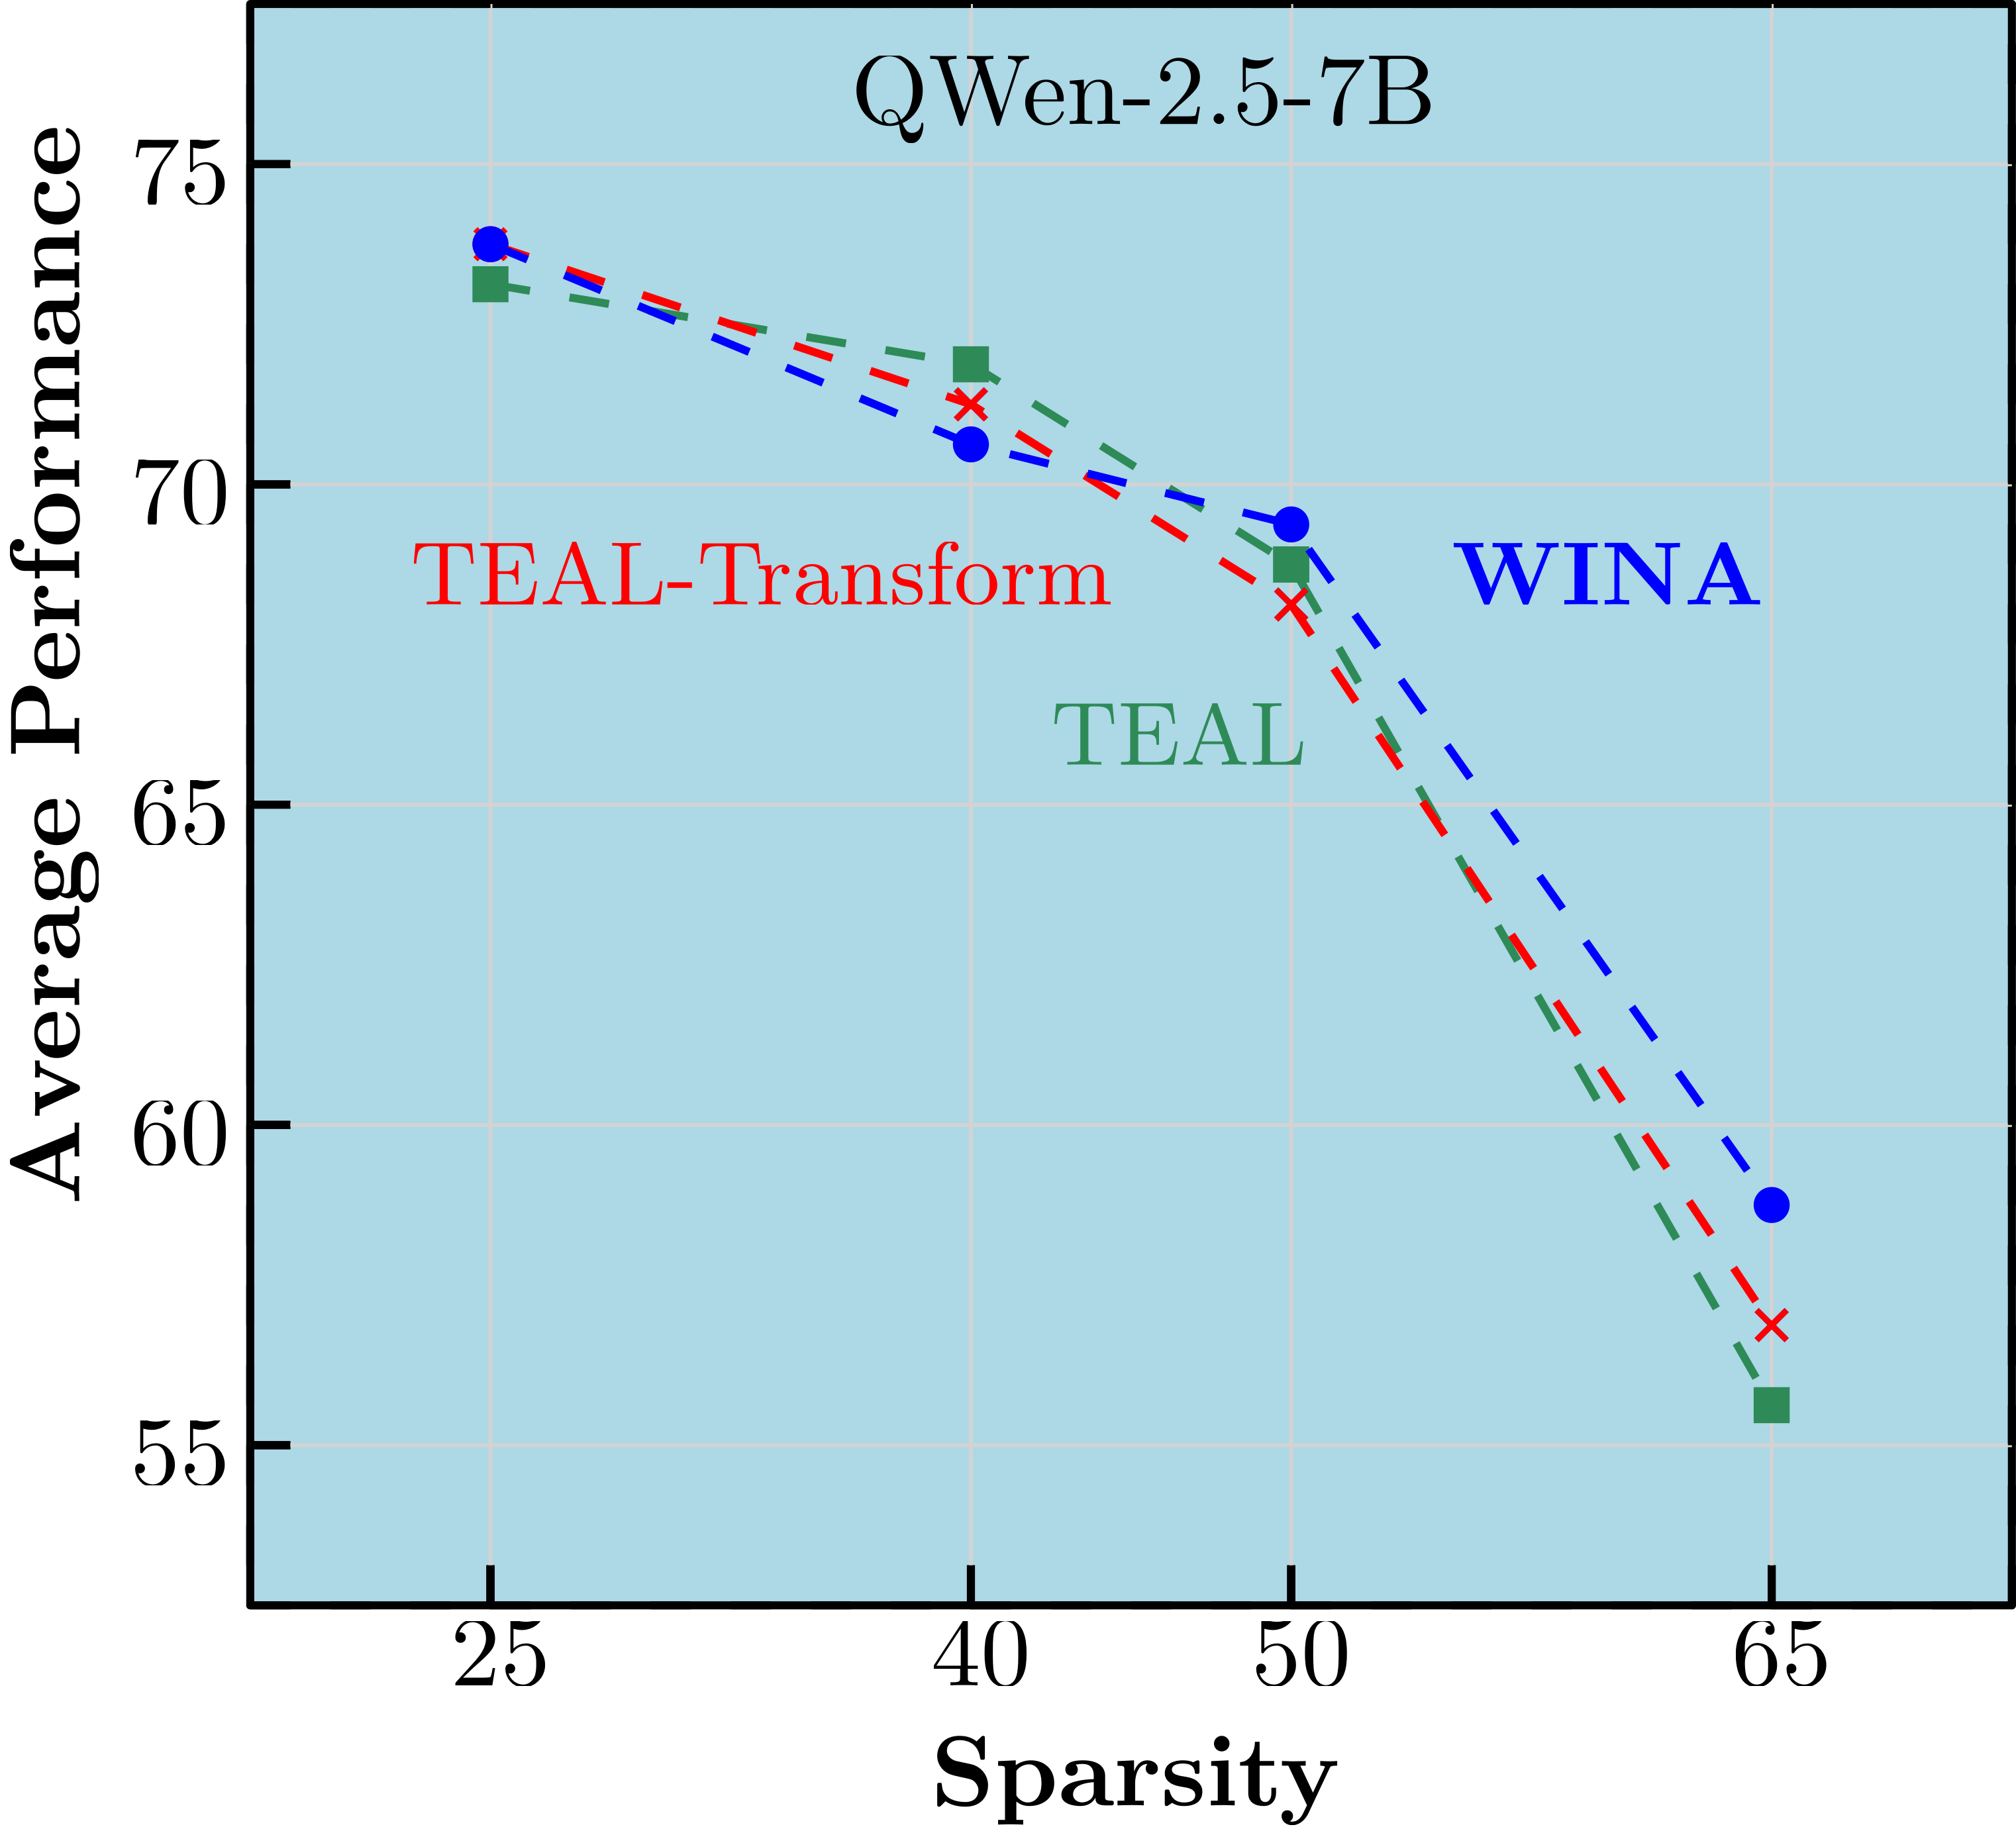
\includegraphics[width=\linewidth]{qwen_2.5_7b.png}
        \caption{QWen-2.5-7B}
        \label{fig:qwen-2.5-7b}
    \end{subfigure}
    \begin{subfigure}[t]{0.24\linewidth}
        \centering        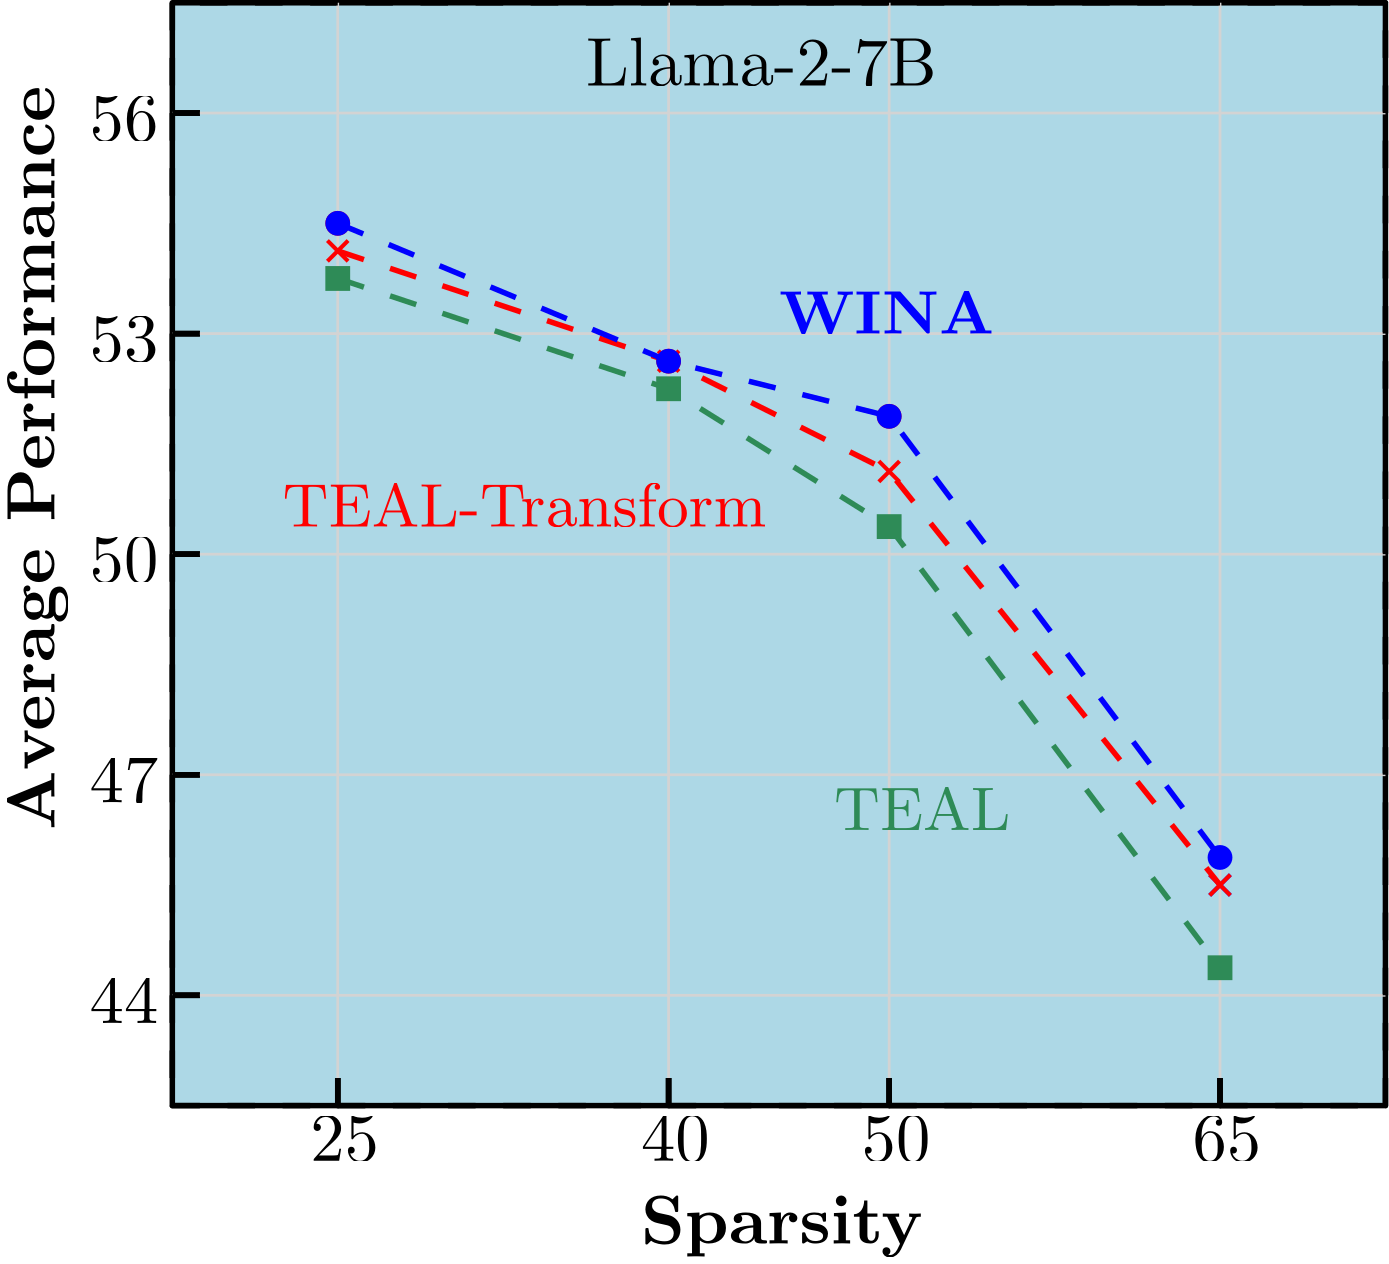
\includegraphics[width=\linewidth]{llama_2_7b.png}
        \caption{Llama-2-7B}
        \label{fig:llama-2-7b}
    \end{subfigure}
    \begin{subfigure}[t]{0.24\linewidth}
        \centering
        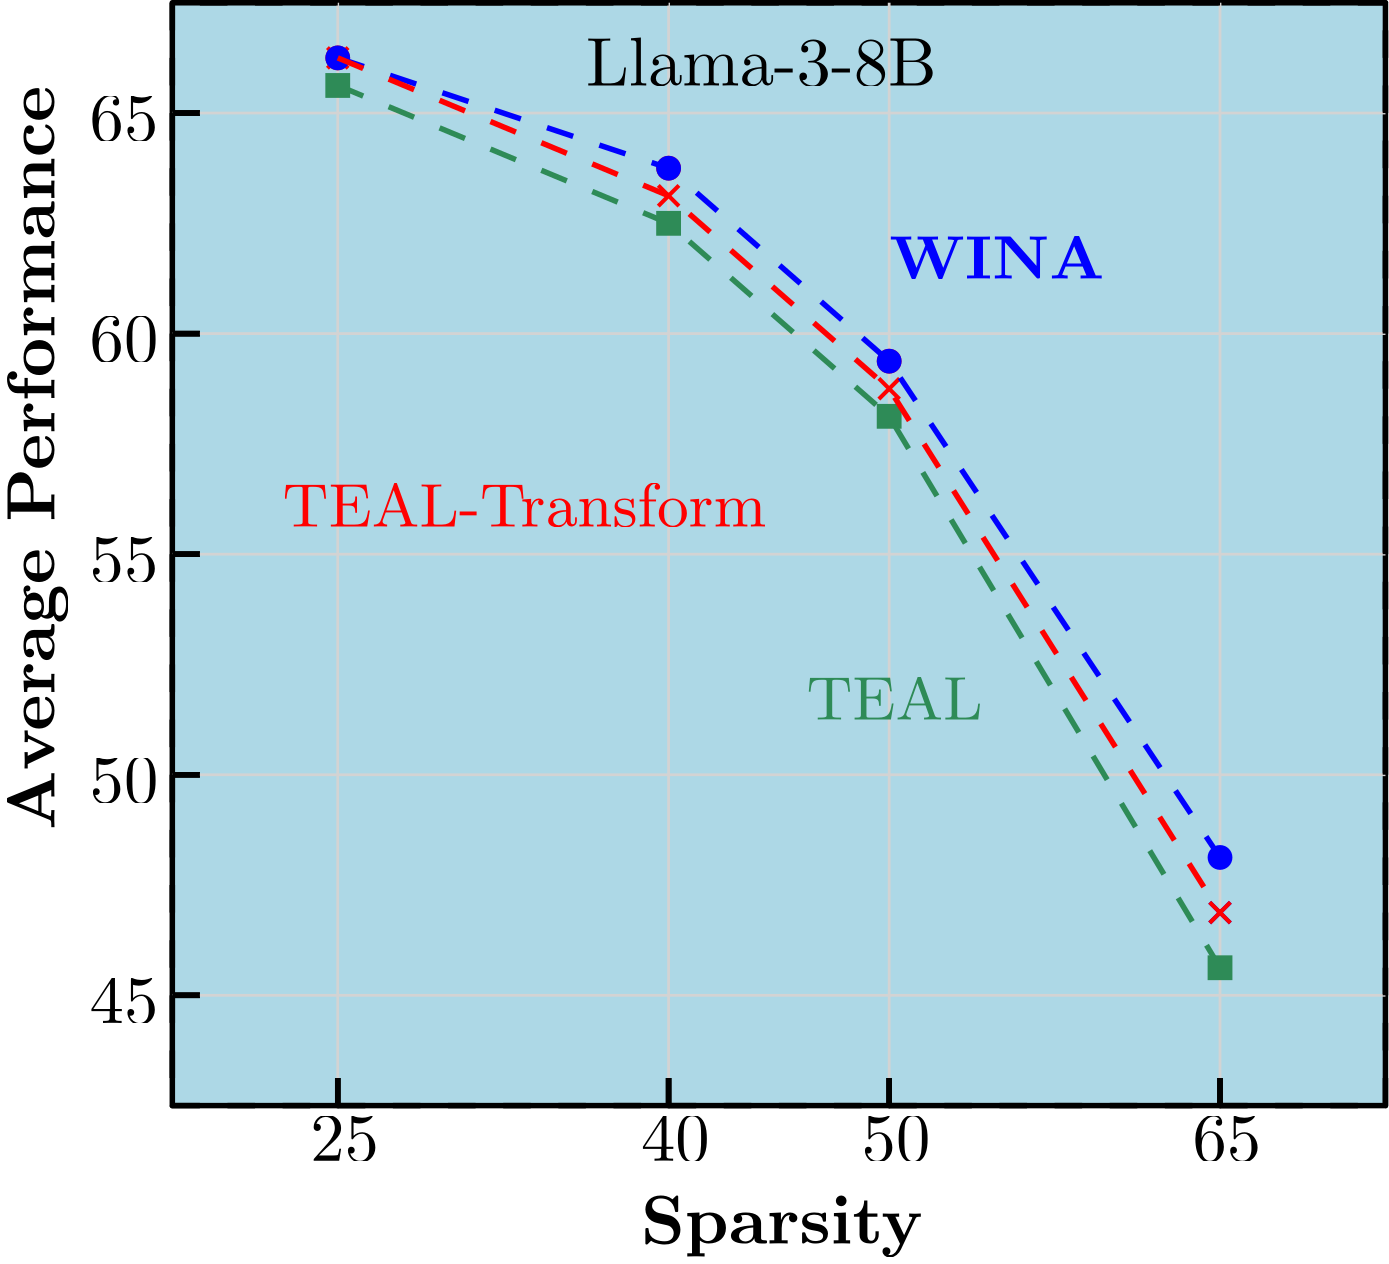
\includegraphics[width=\linewidth]{llama_3_8b.png}
        \caption{Llama-3-8B}
        \label{fig:llama-3-8b}
    \end{subfigure}
    \begin{subfigure}[t]{0.24\linewidth}
        \centering
        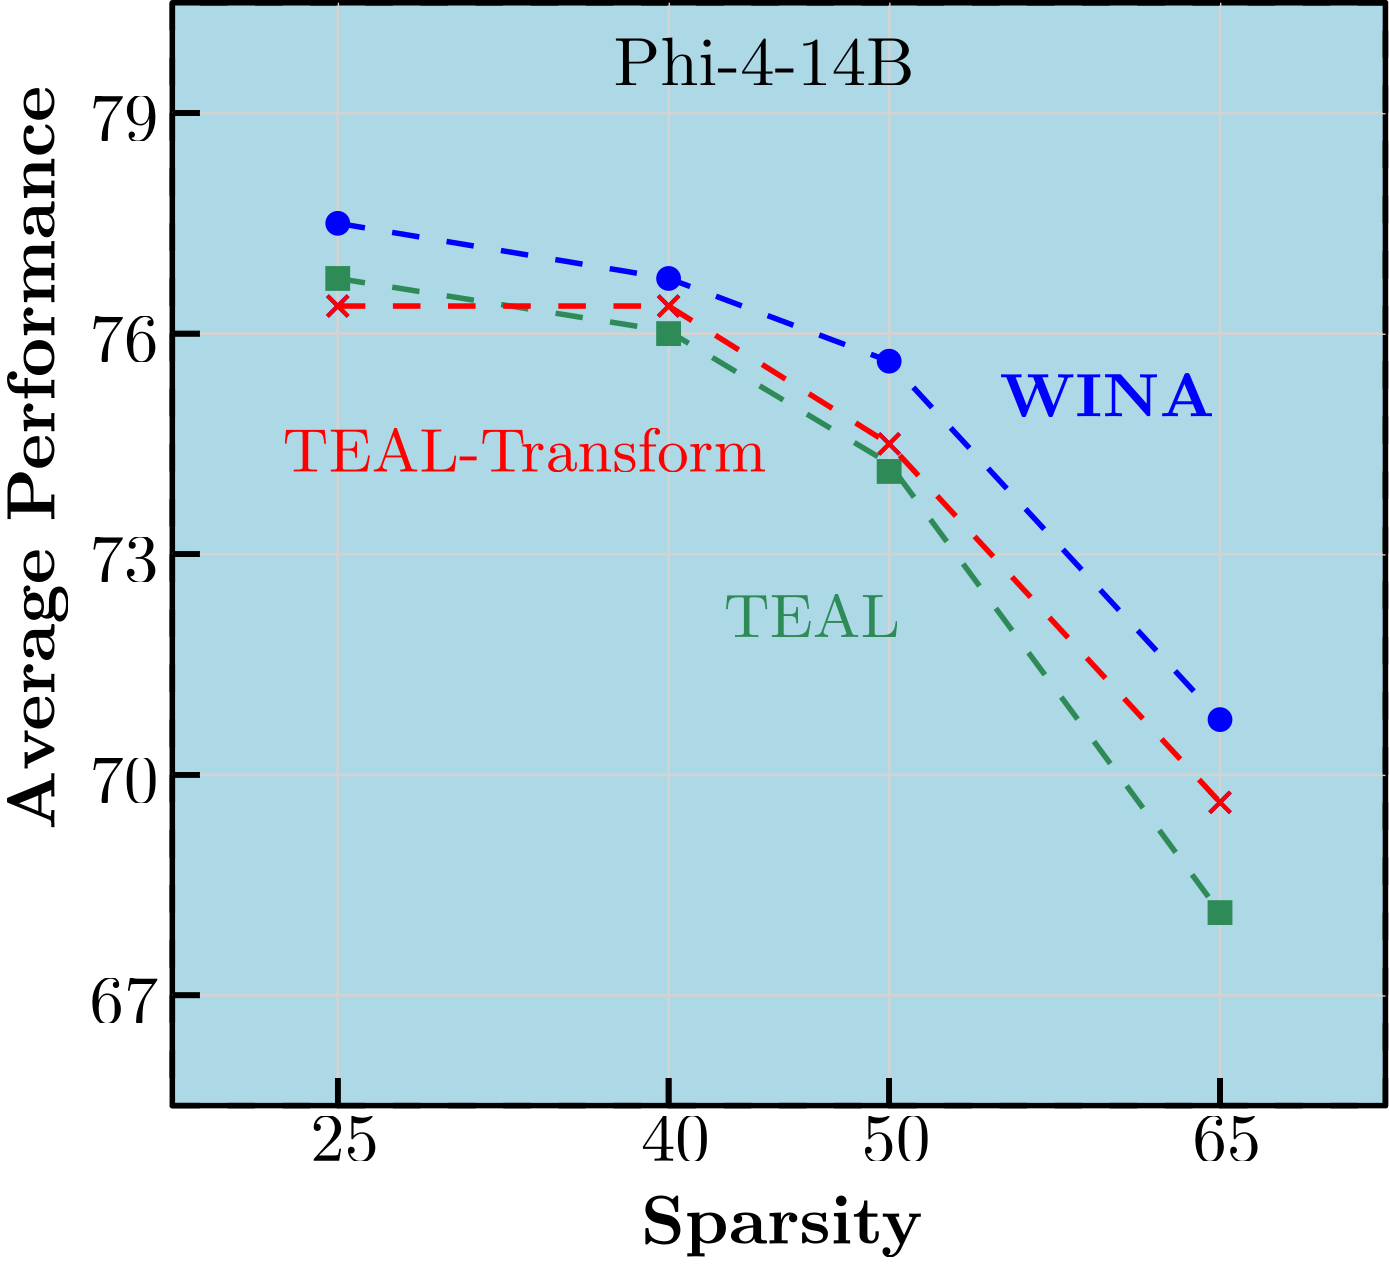
\includegraphics[width=\linewidth]{phi_4_14b.png}
        % \caption{Example caption for Qwen 2.5 7B}
        \caption{Phi-4-14B}
        \label{fig:phi-4-14b}
    \end{subfigure}
    \caption{\textbf{Sparsity-performance frontiers.} Sparsity-performance across Qwen-2.5-7B, Llama-2-7B, Llama-3-8B, and Phi-4-14B.}
    \label{fig:qwen-overview}
\end{figure}

\begin{table*}[t]
  \caption{Results of controlled sparsity experiments over Qwen-2.5-7B}
  \label{tab:qwen25_7b_sparsity}
  \vspace{3pt}
  \centering
  % \addtolength{\tabcolsep}{-1pt}
    \resizebox{1.0\columnwidth}{!}{
\begin{tabular}{llccccccc}
  \toprule[0.1em]
  Method & Sparsity & PiQA & WinoGrande & HellaSwag & Arc-c & MMLU & GSM8K & Avg \\
  \midrule
  Baseline & - & 79.71 & 72.85 & 78.93 & 51.11 & 71.93 & 83.32 & 72.98 \\ \midrule

  \multirow{4}{*}{TEAL~\citep{liu2024trainingfreeactivationsparsitylarge}}  
  & 25\% & 79.27 & 78.56 & 72.77 & 51.19 & 71.30 & 82.87 & {72.83} \\
  & 40\% & 78.40 & 77.28 & 73.09 & 52.65 & 70.20 & 78.32 & \textbf{71.66} \\
  & 50\% & 78.62 & 75.02 & 69.77 & 51.02 & 67.72 & 71.42 & {68.93} \\
  & 65\% & 73.72 & 63.35 & 62.67 & 42.75 & 54.95 & 34.95 & {55.40} \\ \midrule

  \multirow{4}{*}{TEAL-transform} 
  & 25\% & 80.09 & 72.77 & 78.65 & 51.79 & 71.56 & 83.09 & 72.99 \\
  & 40\% & 79.71 & 72.30 & 77.73 & 51.28 & 69.93 & 77.18 & 71.52 \\
  & 50\% & 78.56 & 68.67 & 75.74 & 50.00 & 67.28 & 71.49 & 68.62 \\
  & 65\% & 76.06 & 61.33 & 67.30 & 44.20 & 56.06 & 32.60 & 56.93 \\ \midrule

  \multirow{4}{*}{\algacro{}}  
  & 25\% & 80.05 & 72.69 & 78.58 & 51.37 & 71.51 & 83.93 & \textbf{73.02} \\
  & 40\% & 78.40 & 70.56 & 78.02 & 50.94 & 70.54 & 79.83 & 71.38 \\
  & 50\% & 78.67 & 69.30 & 76.48 & 50.85 & 67.99 & 72.25 & \textbf{69.26} \\
  & 65\% & 76.17 & 61.01 & 70.09 & 42.92 & 59.48 & 38.36 & \textbf{58.34} \\
  \bottomrule[0.1em]
\end{tabular}
  }
\end{table*}

% \begin{table}[t] % [t]表示尽量放在页面顶部
%   \centering
%   \caption{单栏跨栏表格示例}
%   \label{tab:wide}
%   \begin{tabular}{lccr}
%     \toprule
%     Header1 & Header2 & Header3 & Header4 \\
%     \midrule
%     Item1 & 0.25 & 42 & A \\
%     Item2 & 0.67 & 13 & B \\
%     Item3 & 0.92 & 29 & C \\
%     \bottomrule
%   \end{tabular}
% \end{table}
\paragraph{Qwen-2.5-7B.} {We evaluate \algacro{} on Qwen2.5-7B \citep{yang2024qwen2} across various sparsity levels (i.e, 25\% -- 65\%) under the controlled sparsity setting. As shown in \autoref{tab:qwen25_7b_sparsity}, \algacro{} consistently matches or outperforms both TEAL and TEAL -transform across all sparsity levels. Notably, as sparsity increases, the performance gap between \algacro{} and the baselines becomes more pronounced. For instance, at 65\% sparsity, \algacro{} outperforms TEAL by 2.94\% and TEAL-transform by 1.41\% on average. This trend indicates that \algacro{} is more robust under high sparsity, likely due to its ability to retain the most influential activations by jointly considering hidden state magnitudes and weight norms. Particularly on harder tasks such as GSM8K and HellaSwag, \algacro{} maintains relatively strong performance even when aggressive sparsification is applied.}

\begin{table*}[ht]
  \caption{Results of controlled sparsity experiments over Llama-2-7B}
  \vspace{3pt}
  \label{tab:llama2_7b_sparsity}
  \centering
  % \addtolength{\tabcolsep}{-1pt}
    \resizebox{1.0\columnwidth}{!}{
    \begin{tabular}{llccccccc}
  \toprule[0.1em]
  Method & Sparsity & PiQA & Arc-c & WinoGrande & HellaSwag & MMLU & GSM8K & Avg\\
  \midrule
  Baseline & - & 79.05 & 46.33 & 68.98 & 76.00 & 41.82 & 13.87 & 54.34 \\ \midrule

  \multirow{4}{*}{TEAL\,\citep{liu2024trainingfreeactivationsparsitylarge}}  
  & 25\% & 78.18 & 45.99 & 69.85 & 76.01 & 41.30 & 13.34 & 54.11 \\
  & 40\% & 77.53 & 44.45 & 67.88 & 75.32 & 38.66 & 11.07 & 52.49 \\
  & 50\% & 77.53 & 41.21 & 67.25 & 73.57 & 34.71 & 8.79 & 50.51 \\
  & 65\% & 74.43 & 33.87 & 62.12 & 64.20 & 27.05 & 3.56 & 44.21 \\ \midrule

  \multirow{4}{*}{TEAL-transform} 
  & 25\% & 78.45 & 46.42 & 69.14 & 75.93 & 41.75 & 13.42 & 54.19 \\
  & 40\% & 77.69 & 45.48 & 68.43 & 75.18 & 39.22 & 11.05 &  \textbf{52.84} \\
  & 50\% & 78.07 & 43.77 & 66.54 & 73.48 & 36.28 & 10.24 & 51.40 \\
  & 65\% & 74.32 & 37.71 & 63.77 & 66.49 & 29.11 & 3.64 & 45.51 \\ \midrule

  \multirow{4}{*}{\algacro{}}  
  & 25\% & 78.45 & 46.16 & 69.69 & 75.95 & 42.14 & 14.10 & \textbf{54.42} \\
  & 40\% & 77.91 & 45.56 & 67.32 & 75.52 & 39.58 & 11.07 & {52.83} \\
  & 50\% & 78.35 & 44.45 & 67.96 & 73.65 & 36.55 & 9.63 & \textbf{51.76} \\
  & 65\% & 74.59 & 37.88 & 63.93 & 66.55 & 28.81 & 3.18 & \textbf{45.82} \\
  \bottomrule[0.1em]
\end{tabular}
      }
\end{table*}
\paragraph{Llama-2-7B.} {On Llama-2-7B, \algacro{} again shows strong performance under various sparsity constraints. As shown in \autoref{tab:llama2_7b_sparsity}, \algacro{} achieves the highest average accuracy at 25\% sparsity, outperforming both TEAL-based baselines and the full model. While performance naturally degrades at the extreme 65\% sparsity level, \algacro{} still offers the best accuracy, suggesting its robustness under aggressive pruning.}

\begin{table*}
  \caption{Results of controlled sparsity experiments over Llama-3-8B}
  \vspace{3pt}
  \label{tab:llama3_8b_sparsity}
  \centering
  % \addtolength{\tabcolsep}{-1pt}
\resizebox{1.0\columnwidth}{!}{
  \begin{tabular}{llccccccc}
    \toprule[0.1em]
    Method & Sparsity & PiQA & Arc-c & WinoGrande & HellaSwag & MMLU & GSM8K & Avg \\
    \midrule
    Baseline & - & 80.79 & 53.33 & 72.61 & 79.17 & 62.20 & 50.19 & 66.38 \\ \midrule

    % \multirow{4}{*}{TEAL~\citep{liu2024trainingfreeactivationsparsitylarge}}  
    % & 25\% & 80.09 & 53.58 & 72.30 & 78.72 & 61.80 & 50.11 & 66.10 \\
    % & 40\%  & 79.76 & 50.34 & 740\%0 & 77.32 & 59.83 & 42.61 & 63.38 \\
    % & 50\%  & 77.64 & 47.70 & 68.27 & 74.48 & 55.73 & 30.10 & 58.99 \\
    % & 65\% & 72.52 & 37.71 & 60.14 & 58.92 & 33.31 & 3.71  & 44.39 \\ \midrule

\multirow{4}{*}{TEAL~\citep{liu2024trainingfreeactivationsparsitylarge}}  
& 25\% & 80.25 & 53.16 & 73.32 & 78.85 & 61.85 & 48.07 & 65.58 \\
& 40\% & 79.11 & 48.98 & 71.82 & 77.43 & 59.26 & 39.27 & 62.65 \\
& 50\% & 78.24 & 48.12 & 70.01 & 74.83 & 54.50 & 27.37 & 58.51 \\
& 65\% & 73.34 & 37.37 & 63.46 & 61.76 & 32.07 & 4.17 & 45.36 \\ \midrule

    \multirow{4}{*}{TEAL-transform} 
    & 25\% & 80.85 & 53.50 & 73.16 & 78.85 & 61.57 & 47.99 & 65.99 \\
    & 40\%  & 79.43 & 50.60 & 70.88 & 77.36 & 59.23 & 40.11 & 62.94 \\
    & 50\%  & 77.69 & 48.38 & 69.06 & 75.70 & 54.82 & 29.49 & 59.19 \\
    & 65\% & 73.23 & 39.51 & 61.96 & 65.25 & 38.66 & 5.08 & 47.28 \\ \midrule

    \multirow{4}{*}{\algacro{}}  
    & 25\% & 80.79 & 53.16 & 73.24 & 78.96 & 61.54 & 48.29 & \textbf{66.00} \\
    & 40\%  & 79.60 & 50.09 & 71.27 & 77.54 & 58.82 & 41.85 & \textbf{63.20} \\
    & 50\%  & 78.35 & 49.06 & 70.32 & 75.12 & 55.26 & 29.34 & \textbf{59.57} \\
    & 65\% & 73.45 & 40.10 & 62.67 & 64.89 & 38.48 & 7.05 & \textbf{47.77} \\
    \bottomrule[0.1em]
  \end{tabular}
    }
\end{table*}
\paragraph{Llama-3-8B.} The results on Llama-3-8B further emphasize \algacro{}’s resilience to pruning, as summarized in \autoref{tab:llama3_8b_sparsity}. While TEAL slightly outperforms at the 25\% level, \algacro{} leads in all remaining sparsity configurations, culminating in +1.06\% and +2.41\% over TEAL at 50\% sparsity and 65\% sparsity, respectively. Notably, \algacro{} sustains particularly strong performance on reasoning-intensive tasks like GSM8K and ARC Challenge, where other methods show significant drops under compression. These patterns suggest that \algacro{} is not only compression-friendly but also capable of preserving complex decision-making abilities under tight computational budgets.

\begin{table*}
  \caption{Results of controlled sparsity experiments over Phi-4-14B}
  \label{tab:phi4_14b_sparsity}
  \vspace{3pt}
  \centering
  % \addtolength{\tabcolsep}{-1pt}
\resizebox{1.0\columnwidth}{!}{
  \begin{tabular}{llccccccc}
    \toprule[0.1em]
    Method & Sparsity & PiQA & WinoGrande & HellaSwag & Arc-c & MMLU & GSM8K & Avg \\
    \midrule
    Baseline & - & 81.28 & 76.80 & 81.93 & 55.97 & 77.06 & 90.22 & 77.21 \\ \midrule

  \multirow{4}{*}{TEAL~\citep{liu2024trainingfreeactivationsparsitylarge}}  
  & 25\% & 81.07 & 75.45 & 81.92 & 56.23 & 76.63 & 89.84 & 76.86 \\
  & 40\% & 80.79 & 73.80 & 81.21 & 54.95 & 75.10 & 88.02 & 75.98 \\
  & 50\% & 80.63 & 71.98 & 80.06 & 53.84 & 73.52 & 86.13 & 74.36 \\
  & 65\% & 77.64 & 66.06 & 74.26 & 50.77 & 65.17 & 74.37 & 68.71 \\
  \midrule

  \multirow{4}{*}{TEAL-transform} 
  & 25\% & 80.96 & 74.59 & 81.60 & 55.63 & 76.68 & 89.92 & 76.56 \\
  & 40\% & 81.18 & 74.19 & 80.94 & 54.61 & 75.99 & 90.07 & 76.50 \\
  & 50\% & 79.82 & 72.38 & 79.79 & 53.92 & 74.51 & 88.02 & 74.74 \\
  & 65\% & 77.64 & 68.51 & 74.72 & 52.47 & 66.64 & 77.18 & 69.86 \\
  \midrule

\multirow{4}{*}{\algacro{}}  
& 25\% & 81.01 & 75.37 & 81.91 & 56.31 & 76.60 & 90.22 & \textbf{77.57} \\
& 40\% & 81.18 & 72.45 & 81.44 & 56.06 & 76.44 & 90.67 & \textbf{76.71} \\
& 50\% & 81.39 & 73.95 & 81.75 & 54.95 & 75.83 & 87.57 & \textbf{75.91} \\
& 65\% & 78.24 & 70.72 & 77.10 & 51.11 & 70.05 & 77.10 & \textbf{70.72} \\
    \bottomrule[0.1em]
  \end{tabular}
  }
\end{table*}


\paragraph{Phi-4-14B.} \algacro{} also delivers robust performance on Phi-4-14B across all tested sparsity levels, as detailed in \autoref{tab:phi4_14b_sparsity}. It consistently either matches or exceeds the accuracy of both TEAL and TEAL-transform, and achieves the top average score at every sparsity setting. At the highest sparsity of 65\%, for instance, \algacro{} improves upon TEAL and TEAL-transform by +2.01\% and +0.86\%, respectively. Its ability to retain high performance on complex benchmarks such as GSM8K and MMLU, even under severe pruning, highlights its stability. These outcomes demonstrate that \algacro{} can effectively preserve key reasoning mechanisms in large-scale models, making it well-suited for sparsity-constrained deployments.

\begin{table}[H]
\centering
\caption{(G)FLOPs over different sparsity across diffrent model architecture.}\label{tab:gflops}
\begin{tabular}{lcccc}
\toprule
Sparsity & QWen2.5-7B & Llama-2-7B & Llama-3-8B & Phi-4\\
\midrule
Baseline & 7.07 & 6.61 & 7.50 & 14.15  \\
\midrule
0.25 & 5.44 ($\downarrow 23.1\%$) & 4.99 ($\downarrow 24.5\%$) & 5.76 ($\downarrow 23.2\%$) & 10.74($\downarrow 24.1\%$)\\
0.4 &  4.46 ($\downarrow36.9\%$) & 4.02 ($\downarrow39.2\%$) & 4.71 ($\downarrow37.2\%$) & 8.69 ($\downarrow38.6\%$)\\
0.5 & 3.81 ($\downarrow46.1\%$) & 3.37 ($\downarrow49.0\%$) & 4.01 ($\downarrow46.5\%$) & 7.33 ($\downarrow48.2\%$)\\
0.65 & 2.83 ($\downarrow60.0\%$) & 2.40 ($\downarrow63.7\%$) & 2.97 ($\downarrow60.4\%$) & 5.28 ($\downarrow62.7\%$)\\
% \midrule
% {\algacro{} Avg Acc.} & 73.02 & 54.42 & 66.00 & 77.57 \\
\bottomrule
\end{tabular}
\end{table}
\paragraph{Acceleration.} In addition to performance gains, \algacro{} yields substantial computational acceleration across all evaluated LLMs. As shown in~\autoref{tab:gflops}, \algacro{} reduces the overall (G)FLOPs by up to 60.0\% on Qwen-2.5-7B, 63.7\% on Llama-2-7B, 60.4\% on Llama-3-8B, and 62.7\% on Phi-4-14B at the 65\% sparsity level. These consistent reductions in floating point operations could translate to faster inference speeds and lower computational costs, validating \algacro{}’s effectiveness as a practical solution for deployment under tight resource constraints. 
% Notably, these accelerations are achieved without requiring any model retraining, highlighting the plug-and-play nature of our training-free framework.





% \input{src/tab_llama2_13b}
% all results are buged.
% \input{src/tab_mistral_7b}



% \subsection{Empirical Sparsity Analysis.}
\section{Conclusion}\label{sec:conclusion}

In this paper, we introduce \algacro{}, a training-free sparse activation framework that selects active neurons based on both hidden state magnitudes and the column-wise $\ell_2$-norms of subsequent weight matrices. By combining these two signals, \algacro{} addresses key limitations of prior methods such as TEAL, which rely solely on hidden state magnitudes and often suffer from suboptimal sparsity-performance trade-offs and distribution mismatch across layers.

Our theoretical analysis demonstrates that \algacro{} achieves a tighter bound on approximation error compared to existing approaches, under mild assumptions. To bridge the gap between theoretical guarantees and practical deployment in pre-trained LLMs, we further adopted a tensor transformation protocol that enforces column-orthogonality in weight matrices without altering model output.
Our extensive experiments across multiple LLM architectures and benchmarks also validate \algacro{}’s superior performance under controlled sparsity settings, establishing it as a new state-of-the-art in the domain of training-free sparse activation.


% \textbf{Limitations and Future Work.} Our work presents several limitations that warrant discussion. Most notably, the theoretical proof of \algacro{}'s superiority over competing algorithms relies on potentially over-strong assumptions. A key concern is our assumption of independence between weight matrices, which may not fully hold in practice given that all matrices are jointly optimized during pre-training. Future researcha may develope more adaptive criteria selection mechanisms.
% }


% \clearpage
\bibliography{reference}
\bibliographystyle{plain}

\clearpage
\appendix

%\section{Faster matrix multiplication: Full results}

\paragraph{Full table of results.} We provide the best ranks obtained by \method in~\Cref{tab:relaxed-opt-results-appendix}. Overall, we considered 54 matrix multiplication sizes in our experiments. These were chosen roughly representing sizes $\langle m,n,p \rangle$ where $2\leq m,n\leq 5$, with some reasonable cutoff for $p$. Due to symmetries of the underlying matrix multiplication tensor, there exist equivalent algorithms for any permutations of the three axes, hence we focus on sorted sizes $m\leq n\leq p$.

In all but two considered sizes, \method discovered programs which either match or surpass the best known rank. Anecdotally, we encountered some difficulty when increasing the problem size: when we run the discovered programs on sizes beyond $\langle 5,5,5 \rangle$ on 1000 random seeds on evaluators with a single GPU accelerator, we often run out of memory. Hence, extending our setup to larger matrix sizes requires further optimization.

\begin{table}[h]
\rowcolors{2}{white}{gray!30}
\begin{center}
    \scalebox{0.7}{
    \begin{tabular}{ccc}
    $\langle m, n, p \rangle$ & \makecell{best known \\ {[reference]}}  & \method \\ \midrule
    $\langle 2, 2, 2 \rangle$ & 7 \citep{strassen1969gaussian}   & 7   \\ 
    $\langle 2, 2, 3 \rangle$ & 11~\citep{smirnov2013bilinear}& 11 \\ 
    $\langle 2, 2, 4 \rangle$ & 14~\citep{smirnov2013bilinear} & 14 \\ 
    $\langle 2, 2, 5 \rangle$ & 18~\citep{smirnov2013bilinear} & 18 \\ 
    $\langle 2, 2, 6 \rangle$ & 21~\citep{smirnov2013bilinear} & 21 \\ 
    $\langle 2, 2, 7 \rangle$ & 25~\citep{smirnov2013bilinear} & 25 \\ 
    $\langle 2, 2, 8 \rangle$ & 28~\citep{smirnov2013bilinear} & 28 \\ 
    $\langle 2, 2, 9 \rangle$ & 32~\citep{smirnov2013bilinear} & 32 \\ 
    $\langle 2, 2, 10 \rangle$ & 35~\citep{smirnov2013bilinear} & 35 \\ 
    $\langle 2, 2, 11 \rangle$ & 39~\citep{smirnov2013bilinear} & 39 \\ 
    $\langle 2, 2, 12 \rangle$ & 42~\citep{smirnov2013bilinear} & 42 \\ 
    $\langle 2, 2, 13 \rangle$ & 46~\citep{smirnov2013bilinear} & 46 \\ 
    $\langle 2, 2, 14 \rangle$ & 49~\citep{smirnov2013bilinear} & 49 \\ 
    $\langle 2, 2, 15 \rangle$ & 53~\citep{smirnov2013bilinear} & 53 \\ 
    $\langle 2, 2, 16 \rangle$ & 56~\citep{smirnov2013bilinear} & 56 \\ 
    $\langle 2, 3, 3 \rangle$ & 15~\citep{smirnov2013bilinear} & 15 \\ 
    $\langle 2, 3, 4 \rangle$ & 20~\citep{smirnov2013bilinear} & 20 \\ 
    $\langle 2, 3, 5 \rangle$ & 25~\citep{smirnov2013bilinear} & 25 \\ 
    \end{tabular}
    }
    \scalebox{0.7}{
    \begin{tabular}{ccc}
    $\langle m, n, p \rangle$ & \makecell{best known \\ {[reference]}}  & \method \\ \midrule
    $\langle 2, 3, 6 \rangle$ & 30~\citep{smirnov2013bilinear} & 30 \\ 
    $\langle 2, 3, 7 \rangle$ & 35~\citep{smirnov2013bilinear} & 35 \\ 
    $\langle 2, 3, 8 \rangle$ & 40~\citep{smirnov2013bilinear} & 40 \\ 
    $\langle 2, 3, 9 \rangle$ & 45~\citep{smirnov2013bilinear} & 45 \\ 
    $\langle 2, 3, 10 \rangle$ & 50~\citep{smirnov2013bilinear} & 50 \\ 
    $\langle 2, 4, 4 \rangle$ & 26~\citep{smirnov2013bilinear} & 26 \\ 
    $\langle 2, 4, 5 \rangle$ & 33~\citep{hopcroft} & \textcolor{darkgreen}{\textbf{32}} \\
    $\langle 2, 4, 6 \rangle$ & 39~\citep{smirnov2013bilinear} & 39 \\ 
    $\langle 2, 4, 7 \rangle$ & 46~\citep{smirnov2013bilinear} & \textcolor{darkgreen}{\textbf{45}} \\
    $\langle 2, 4, 8 \rangle$ & 52~\citep{smirnov2013bilinear} & \textcolor{darkgreen}{\textbf{51}} \\
    $\langle 2, 5, 5 \rangle$ & 40~\citep{smirnov2013bilinear} & 40 \\ 
    $\langle 2, 5, 6 \rangle$ & 48~\citep{smirnov2013bilinear} & \textcolor{darkgreen}{\textbf{47}} \\ 
    $\langle 3, 3, 3 \rangle$ & 23~\citep{laderman}   & 23   \\
    $\langle 3, 3, 4 \rangle$ & 29~\citep{smirnov2013bilinear} & 29 \\ 
    $\langle 3, 3, 5 \rangle$ & 36~\citep{smirnov2013bilinear} & 36 \\ 
    $\langle 3, 3, 6 \rangle$ & 40~\citep{smirnov2013bilinear} & 40 \\ 
    $\langle 3, 3, 7 \rangle$ & 49~\citep{smirnov2013bilinear} & 49 \\ 
    $\langle 3, 3, 8 \rangle$ & 55~\citep{smirnov2013bilinear} & 55 \\ 
    \end{tabular}
    }
    \scalebox{0.7}{
    \begin{tabular}{ccc}
    $\langle m, n, p \rangle$ & \makecell{best known \\ {[reference]}}  & \method \\ \midrule
    $\langle 3, 4, 4 \rangle$ & 38~\citep{smirnov2013bilinear} & 38 \\ 
    $\langle 3, 4, 5 \rangle$ & 47~\citep{fawzi2022discovering} & 47 \\ 
    $\langle 3, 4, 6 \rangle$ & 56~\citep{Kauers_2025} & \textcolor{darkgreen}{\textbf{54}} \\ 
    $\langle 3, 4, 7 \rangle$ & 66~\citep{smirnov2021} & \textcolor{darkgreen}{\textbf{63}} \\ 
    $\langle 3, 4, 8 \rangle$ & 75~\citep{smirnov2021}   & \textcolor{darkgreen}{\textbf{74}} \\ 
    $\langle 3, 5, 5 \rangle$ & 58~\citep{smirnov2021} & 58 \\ 
    $\langle 3, 5, 6 \rangle$ & 70~\citep{Kauers_2025} & \textcolor{darkgreen}{\textbf{68}} \\
    $\langle 3, 5, 7 \rangle$ & 82~\citep{smirnov2021} & \textcolor{darkgreen}{\textbf{80}} \\ 
    $\langle 4, 4, 4 \rangle$ & 49~\citep{strassen1969gaussian} & \textcolor{darkgreen}{\textbf{48}}  \\ 
    $\langle 4, 4, 5 \rangle$ & 62~\citep{kauers2023flip}   & \textcolor{darkgreen}{\textbf{61}}    \\
    $\langle 4, 4, 6 \rangle$ & 73~\citep{Kauers_2025} & 73 \\ 
    $\langle 4, 4, 7 \rangle$ & 87~\citep{smirnov2013bilinear,strassen1969gaussian} & \textcolor{darkgreen}{\textbf{85}}    \\
    $\langle 4, 4, 8 \rangle$ & 98~\citep{strassen1969gaussian} & \textcolor{darkgreen}{\textbf{96}} \\ 
    $\langle 4, 4, 9 \rangle$ & 104~\citep{smirnov2022} & \textcolor{purple}{108} \\ 
    $\langle 4, 5, 5 \rangle$ & 76~\citep{fawzi2022discovering} & 76 \\ 
    $\langle 4, 5, 6 \rangle$ & 93~\citep{Kauers_2025}   & \textcolor{darkgreen}{\textbf{90}} \\ 
    $\langle 5, 5, 5 \rangle$ & 93~\citep{flip_graphs_with_symmetry} & 93 \\ 
    $\langle 6, 6, 6 \rangle$ & 153~\citep{flip_graphs_with_symmetry} & \textcolor{purple}{156} \\ 
    \end{tabular}
    }
\caption{Full version of \Cref{tab:relaxed-opt-results}, showing the best ranks obtained by \method for tensor decomposition for all considered parameters. Of the 54 targets, \method matches the state of the art in 38 cases, surpasses it in 14 cases (green), and falls behind in 2 cases (red). In all cases, \method provides exact algorithms, using integer or half-integer entries in the decomposition. For $\langle 3, 4, 7\rangle$, $\langle 4, 4, 4\rangle$, and $\langle 4, 4, 8\rangle$, the algorithms discovered by \method use complex-valued multiplications which can be used for exact multiplication of complex or real-valued matrices. The decompositions shown in this table can be found in \ResultsColab.}
    \label{tab:relaxed-opt-results-appendix}
\end{center}
\end{table}

\emph{Note}: Concurrent work~\cite{kauers2025consequences} has also found a rank-$90$ algorithm for $\langle 4, 5, 6 \rangle$.

\paragraph{Magnified version of \Cref{fig:relaxed-opt-diff} (left).} In \Cref{fig:relaxed-opt-diff-appendix-1,fig:relaxed-opt-diff-appendix-2,fig:relaxed-opt-diff-appendix-3}, we show a magnified version of \Cref{fig:relaxed-opt-diff} (left), which corresponds to the program that discovers a decomposition of rank 48 for the 3D tensor representing the operation of multiplying two $4\times 4$ matrices. 

\begin{figure}[p]
\renewcommand{\thefigure}{\arabic{figure}a}\vspace{-0.03\textwidth}
\begin{adjustbox}{width=0.9\textwidth}
\begin{minipage}{0.9\textwidth}
\begin{lstlisting}[style=pydiff, backgroundcolor=\color{backcolour}]
@@ -45,9 +45,14 @@
   # EVOLVE-BLOCK-START
   def _get_optimizer(self) -> optax.GradientTransformation:
     """Returns optimizer."""
-    return optax.adam(self.hypers.learning_rate)
+    return optax.adamw(
+        self.hypers.learning_rate, weight_decay=self.hypers.weight_decay
+    )
 
   def _get_init_fn(self) -> jax.nn.initializers.Initializer:
     """Returns initializer function."""
-    return initializers.normal(0.0, self.hypers.init_scale, jnp.complex64)
+    # Initialize with a smaller scale to encourage finding low-rank solutions.
+    # Increase scale slightly for better exploration.
+    scale = self.hypers.init_scale
+    return initializers.normal(0 + 1j * 0, scale * 0.2, jnp.complex64)

@@ -80,6 +85,66 @@
     # Gradient updates.
     updates, opt_state = self.opt.update(grads, opt_state, decomposition)
     decomposition = optax.apply_updates(decomposition, updates)
+    # Add a small amount of gradient noise to help with exploration
+    rng, g_noise_rng = jax.random.split(rng)
+    decomposition = jax.tree_util.tree_map(
+        lambda x: x
+        + self.hypers.grad_noise_std * jax.random.normal(g_noise_rng, x.shape),
+        decomposition,
+    )
+
+    # Add noise to the decomposition parameters (exploration).
+    _, noise_rng = jax.random.split(rng)
+    noise_std = self._linear_schedule(
+        global_step, start=self.hypers.noise_std, end=0.0
+    )
+    decomposition = jax.tree_util.tree_map(
+        lambda x: x + noise_std * jax.random.normal(noise_rng, x.shape),
+        decomposition,
+    )
+
+    # Cyclical annealing for clipping threshold.
+    cycle_length = 2000  # Number of steps per cycle
+    cycle_progress = (
+        global_step % cycle_length
+    ) / cycle_length  # Normalized progress within the current cycle [0, 1)
+
+    # Map cycle progress to a sinusoidal curve. Ranges from 0 to 1.
+    clip_threshold_multiplier = (1 + jnp.cos(2 * jnp.pi * cycle_progress)) / 2
+
+    clip_threshold = self.hypers.clip_min + clip_threshold_multiplier * (
+        self.hypers.clip_max - self.hypers.clip_min
+    )
+
+    def soft_clip(x, threshold):
+      # Clipping the real and imaginary parts separately.
+      x_re = jnp.real(x)
+      x_im = jnp.imag(x)
+
+      x_re_clipped = jnp.where(
+          x_re > threshold, threshold + (x_re - threshold) * 0.1, x_re
+      )
+      x_re_clipped = jnp.where(
+          x_re_clipped < -threshold,
+          -threshold + (x_re_clipped + threshold) * 0.1,
+          x_re_clipped,
+      )
\end{lstlisting}
\end{minipage}
\end{adjustbox}
\caption{
Magnified version of~\Cref{fig:relaxed-opt-diff}(left), giving the program that discovers a faster algorithm to multiply $4\times4$ matrices (\emph{1/3}).}\label{fig:relaxed-opt-diff-appendix-1}
\centering
\end{figure}
\addtocounter{figure}{-1}


\begin{figure}[p]
\renewcommand{\thefigure}{\arabic{figure}b}\vspace{-0.03\textwidth}
\begin{adjustbox}{width=0.9\textwidth}
\begin{minipage}{0.9\textwidth}
\begin{lstlisting}[style=pydiff, backgroundcolor=\color{backcolour}, firstnumber=66]
+
+      x_im_clipped = jnp.where(
+          x_im > threshold, threshold + (x_im - threshold) * 0.1, x_im
+      )
+      x_im_clipped = jnp.where(
+          x_im_clipped < -threshold,
+          -threshold + (x_im_clipped + threshold) * 0.1,
+          x_im_clipped,
+      )
+
+      return x_re_clipped + 1j * x_im_clipped
+
+    decomposition = jax.tree_util.tree_map(
+        lambda x: soft_clip(x, clip_threshold), decomposition
+    )
+
     return decomposition, opt_state, loss
 
   def _loss_fn(
@@ -91,13 +156,86 @@
     """Computes (batched) loss on learned decomposition."""
     # Compute reconstruction loss.
     rec_tensor = self._decomposition_to_tensor(decomposition)  # (B, N, M, P)
+
+    # Add noise to the target tensor (robustness).
+    rng, noise_rng = jax.random.split(rng)
+    target_noise = self.hypers.target_noise_std * jax.random.normal(
+        noise_rng, self.target_tensor.shape
+    )
+    noisy_target_tensor = self.target_tensor + target_noise
+
+    # Hallucination loss (encourages exploration by randomly replacing values)
+    hallucination_prob = self.hypers.hallucination_prob
+    hallucination_scale = self.hypers.hallucination_scale
+
+    def hallucinate(x, hallucination_rng):
+      mask = jax.random.bernoulli(hallucination_rng, p=hallucination_prob)
+      noise = hallucination_scale * jax.random.normal(
+          hallucination_rng, x.shape
+      )
+      return jnp.where(mask, noise, x)
+
+    _, factor_rng = jax.random.split(rng)
+    decomposition = jax.tree_util.tree_map(
+        lambda x: hallucinate(x, jax.random.split(factor_rng)[0]),
+        decomposition,
+    )
+
     # Add a batch dimension to `target_tensor` to ensure correct broadcasting.
     # Define the loss as the L2 reconstruction error.
-    rec_loss = l2_loss_complex(self.target_tensor[None, ...], rec_tensor)
+    rec_loss = l2_loss_complex(noisy_target_tensor[None, ...], rec_tensor)
 
     # We must return a real-valued loss.
-    return jnp.real(rec_loss)
 
+    # Discretization loss (encourage entries to be multiples of 1/2 or integer).
+    def dist_to_half_ints(x):
+      x_re = jnp.real(x)
+      x_im = jnp.imag(x)
+      return jnp.minimum(
+          jnp.abs(x_re - jnp.round(x_re * 2) / 2),
+          jnp.abs(x_im - jnp.round(x_im * 2) / 2),
+      )
+
\end{lstlisting}
\end{minipage}
\end{adjustbox}
\caption{Magnified version of~\Cref{fig:relaxed-opt-diff}(left), giving the program that discovers a faster algorithm to multiply $4\times4$ matrices  (\emph{2/3}).}\label{fig:relaxed-opt-diff-appendix-2}
\centering
\end{figure}
\addtocounter{figure}{-1}


\begin{figure}[p]
\renewcommand{\thefigure}{\arabic{figure}c}\vspace{-0.03\textwidth}
\begin{adjustbox}{width=0.9\textwidth}
\begin{minipage}{0.9\textwidth}
\begin{lstlisting}[style=pydiff, backgroundcolor=\color{backcolour}, firstnumber=131]
+    def dist_to_ints(x):
+      return jnp.abs(x - jnp.round(x))
+
+    discretization_loss = 0.0
+    for factor in decomposition:
+      discretization_loss += jnp.mean(dist_to_half_ints(factor))
+      discretization_loss += jnp.mean(dist_to_ints(factor))
+
+    discretization_loss /= (
+        len(decomposition) * 2
+    )  # average across all factors and loss components
+
+    discretization_weight = self._linear_schedule(
+        global_step, start=0.0, end=self.hypers.discretization_weight
+    )
+
+    # Cosine annealing for half-integer loss.
+    cycle_length = self.config.training_steps // 4  # Number of steps per cycle
+    cycle_progress = (
+        global_step % cycle_length
+    ) / cycle_length  # Normalized progress within the current cycle [0, 1)
+    half_int_multiplier = (1 + jnp.cos(jnp.pi * cycle_progress)) / 2
+    half_int_multiplier = (
+        1 - self.hypers.half_int_start
+    ) * half_int_multiplier + self.hypers.half_int_start
+
+    total_loss = (
+        rec_loss
+        + discretization_weight * discretization_loss * half_int_multiplier
+    )
+
+    # Add penalty for large values (stability).
+    large_value_penalty = 0.0
+    for factor in decomposition:
+      large_value_penalty += jnp.mean(jnp.abs(factor) ** 2)
+    large_value_penalty /= len(decomposition)
+    total_loss += self.hypers.large_value_penalty_weight * large_value_penalty
+
+    return jnp.real(total_loss)
+
 
 def l2_loss_complex(x: jnp.ndarray, y: jnp.ndarray) -> jnp.ndarray:
   """Elementwise L2 loss for complex numbers."""
@@ -117,6 +255,18 @@
   return hyper.zipit([
-      hyper.uniform('init_scale', hyper.interval(0.2, 1.5)),
-      hyper.uniform('learning_rate', hyper.interval(0.05, 0.3)),
+      hyper.uniform('init_scale', hyper.interval(0.1, 1.0)),
+      hyper.uniform('learning_rate', hyper.interval(0.01, 0.2)),
+      hyper.uniform('discretization_weight', hyper.interval(0.0, 0.1)),
+      hyper.uniform('hallucination_prob', hyper.interval(0.0, 0.2)),
+      hyper.uniform('hallucination_scale', hyper.interval(0.0, 0.2)),
+      hyper.uniform('noise_std', hyper.interval(0.0, 0.01)),
+      hyper.uniform('target_noise_std', hyper.interval(0.0, 0.01)),
+      hyper.uniform('weight_decay', hyper.interval(0.00001, 0.001)),
+      hyper.uniform('clip_min', hyper.interval(0.0, 0.5)),
+      hyper.uniform('clip_max', hyper.interval(1.0, 3.0)),
+      hyper.uniform('large_value_penalty_weight', hyper.interval(0.0, 0.01)),
+      # Add noise to the gradient to aid in exploration.
+      hyper.uniform('grad_noise_std', hyper.interval(0.0, 0.001)),
+      hyper.uniform('half_int_start', hyper.interval(0.0, 1.0)),
   ])
 # EVOLVE-BLOCK-END
\end{lstlisting}
\end{minipage}
\end{adjustbox}
\caption{Magnified version of~\Cref{fig:relaxed-opt-diff}(left), giving the program that discovers a faster algorithm to multiply $4\times4$ matrices  (\emph{3/3}). Here \texttt{hyper} is a user-provided library for generating hyperparameter sweeps.}\label{fig:relaxed-opt-diff-appendix-3}
\centering
\end{figure}

\clearpage
\section{Details of mathematical discoveries of \method}\label{app:maths}

The data and verification code for all constructions reported in this section appear in \ResultsColab.

\subsection{First autocorrelation inequality}
For any function $f: \mathbb{R} \rightarrow \mathbb{R}$, define the \emph{autoconvolution} of $f$ as $$f*f (t) \coloneqq \int_\mathbb{R} f(t-x) f(x)\ dx.$$
Let $C_1$ denote the largest constant satisfying
\begin{equation}\label{maxf}
 \max_{-1/2 \leq t \leq 1/2} f*f(t) \geq C_1 \left(\int_{-1/4}^{1/4} f(x)\ dx\right)^2
\end{equation}
for all non-negative $f: \mathbb{R} \rightarrow \mathbb{R}$.  This problem arises in additive combinatorics, relating to the size of Sidon sets.  It is currently known that
$$1.28 \leq C_1 \leq 1.5098,$$
with the lower bound achieved in \cite{cloninger2017suprema} and the upper bound achieved in \cite{matolcsi2010improved} via a step function construction.
\method found a step function with 600 equally-spaced intervals on $[-1/4,1/4]$ that gives a slightly better upper bound $C_1 \leq 1.5053$.

\subsection{Second autocorrelation inequality}
Let $C_2$ be the smallest constant for which one has
$$ \|f*f\|_2^2 \leq C_2 \|f*f\|_1 \|f*f\|_\infty$$
for all non-negative $f:\mathbb{R} \rightarrow \mathbb{R}$.
It is known that
$$ 0.88922 \leq C_2 \leq 1$$
with the lower bound coming from a step function construction \cite{matolcsi2010improved}. 
\method found a step function with 50 equally-spaced intervals on $[-1/4,1/4]$ that gives a slightly better lower bound $0.8962 \leq C_2$.

\subsection{Third autocorrelation inequality}
Let $C_3$ be the largest constant satisfying
$$ \max_{-1/2 \leq t \leq 1/2} \left|f*f(t)\right| \geq C_3 \left(\int_{-1/4}^{1/4} f(x)\ dx\right)^2$$
for any function $f: \mathbb{R}  \rightarrow \mathbb{R}$. Clearly $C_3 \leq C_1$, since we now allow $f$ to take positive and negative values.  
There is a step function that gives the upper bound $C_3 \leq 1.45810$ \cite[page 75]{vinuesa2010generalized}.
\method found a step function with 400 equally-spaced intervals on $[-1/4,1/4]$ that gives a slightly better upper bound $C_3 \leq 1.4557$.


\subsection{An uncertainty inequality}

Given a function $f: \mathbb{R} \to \mathbb{R}$, define the Fourier transform $\hat f(\xi) := \int_\mathbb{R} f(x) e^{-2\pi i x\xi}\ dx$ and
$$ A(f) := \inf \{r > 0: f(x) \geq 0 \hbox{ for all } |x| \geq r \}.$$
Let $C_4$ be the largest constant for which one has
$$ A(f) A(\hat f) \geq C_4$$
for all even $f$ with $\max(f(0), \hat f(0)) < 0$.  It is known~\cite{gonccalves2017hermite} that
$$ 0.2025 \leq C_4 \leq 0.3523.$$
(The upper bound is stated as $0.353$ in the paper, but rounding their solution to the fourth digit gives $0.3523$).
We improved the upper bound to $C_4 \leq 0.3521$ with a similar linear combination as in~\cite{gonccalves2017hermite}, but with refined constants that were found by \method.

To obtain upper bounds for $C_4$, one constructs a specific "test function" $f$ satisfying the conditions and calculates the value $A(f)A(\hat f)$ for this function, which provides an upper bound $C_4 \le A(f)A(\hat f)$. Following the approach in~\cite{gonccalves2017hermite}, the test function is sought in the form $f(x) = P(x)e^{-\pi x^2}$, where $P(x)$ is an even polynomial constructed as a linear combination of Hermite polynomials $H_{4k}(x)$. This form is particularly useful because the Fourier transform of $H_n(x)e^{-\pi x^2}$ is $i^n H_n(\xi)e^{-\pi \xi^2}$. For an even polynomial $P(x) = \sum c_{4k} H_{4k}(x)$, the Fourier transform of $f(x)$ is $\hat f(\xi) = \sum c_{4k} i^{4k} H_{4k}(\xi)e^{-\pi \xi^2} = (\sum c_{4k} H_{4k}(\xi))e^{-\pi \xi^2} = P(\xi)e^{-\pi \xi^2}$. Thus, $A(f)$ is related to the largest positive root of $P(x)$, and $A(\hat f)$ is related to the largest positive root of $P(\xi)$. Specifically, if $P(x) \ge 0$ for large $|x|$, $A(f)$ is the largest positive root of $P(x)$, and $A(\hat f)$ is the largest positive root of $P(\xi)$, implying $A(f) = A(\hat f)$. The inequality becomes $C_4 \le (A(f))^2$.

The method involves finding coefficients $c_0, c_1, c_2, \dots$ for the polynomial $P(x) = c_0 H_0(x) + c_1 H_4(x) + c_2 H_8(x) + \dots$ such that $P(x)$ satisfies certain constraints (related to $f(0)<0, \hat f(0)<0$ and being positive for large $|x|$) and minimizes the largest positive root of $P(x)$. In our approach, the polynomial $P(x)$ is constructed such that $P(0)=0$ (a condition used in the optimization process to simplify constraints), meaning $P(x)$ has a factor of $x^2$. The largest positive root $r_{\max}$ of $P(x)$ is then the largest positive root of $P(x)/x^2$. The upper bound on $C_4$ derived from this construction is $r_{\max}^2 / (2\pi)$.

The refined constants found by \method for $P(x) = c_0 H_0(x) + c_1 H_4(x) + c_2 H_8(x)$ are $[c_0, c_1, c_2] \approx [0.32925, -0.01159, -8.9216 \times 10^{-5}]$. Using these coefficients to construct $P(x)$, finding its largest positive root $r_{\max}$ (by finding the largest positive root of $P(x)/x^2$), and calculating $r_{\max}^2 / (2\pi)$ yields the improved upper bound $C_4 \leq 0.3521$. Qualitatively our linear combination is very similar to the one found in~\cite{gonccalves2017hermite}, thus empirically confirming their hypothesis the construction is nearly optimal.

\emph{Note}: After publishing the first version of this manuscript, Henry Cohn pointed out that in a recent paper~\cite{cohn2019optimal} they used a similar, but more refined approach to get the better constant 0.3284. By incorporating their refined approach into \method, we improved our reported constant further to 0.3216. For details, we refer to \ResultsColab.


\subsection{Erd\H{o}s' minimum overlap problem}
Let $C_5$ be the largest constant for which
$$ \sup_{x \in [-2,2]} \int_{-1}^1 f(t) g(x+t)\ dt\geq C_5$$
for all non-negative $f,g: [-1,1] \to [0,1]$ with $f+g=1$ on $[-1,1]$ and $\int f = 1$, where we extend $f,g$ by zero outside of $[-1,1]$. This constant controls the asymptotics of the Minimum Overlap Problem of \cite{erdHos1955some}.  The bounds
$$ 0.379005 \leq C_5 \leq 0.380927$$
are known, where the lower bound was obtained in \cite{white2023new} via convex programming methods.

It is known (see~\cite{haugland2016minimum}) that
this constant is equal to the infimum, over all step
functions $h$ on $[0, 2]$ with values in $[0, 1]$ and satisfying
$
\int_0^2 h(x)dx = 1
$
of
$$
\max_k \int h(x)(1 - h(x+k))dx 
.$$ The upper bound to the Erd\H{o}s minimum overlap problem was then obtained by using this result, in~\cite{haugland2016minimum} by a step function
construction. The step function depicted in \Cref{fig:erdos} does ever so slightly better than the previous bound, giving the upper bound of $C_5 \leq 0.380924$.

\begin{figure}
    \centering
    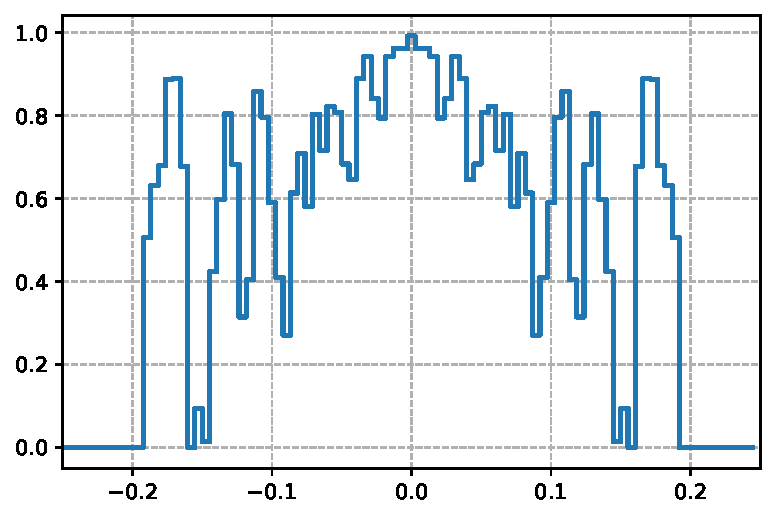
\includegraphics[scale=0.5]{figures/erdos_min_overlap.pdf}
    \caption{Construction found by \method for the minimum overlap problem of Erd\H{o}s.}
    \label{fig:erdos}
\end{figure}


~

\subsection{Sums and differences of finite sets}
Let $C_6$ be the largest constant for which the following statement holds: there exist arbitrarily large finite sets of integers $A,B$ with $|A+B| \ll |A|$ and $|A-B| \gg |A+B|^{C_6}$.
(Here $A+B = \{a+b : a \in A, b \in B\}$ and $A-B = \{a-b : a \in A, b \in B\}$ denote the sumset and difference set, respectively. The notation $X \ll Y$ means that $X \le C Y$ for some constant $C$ independent of the sets $A,B$ (for sufficiently large sets $A,B$). The notation $X \gg Y$ means that $X \ge C' Y$ for some positive constant $C'$ independent of the sets $A,B$ (for sufficiently large sets $A,B$).)
\begin{equation}\label{cds}
 1.14465 \leq C_6 \leq \frac{4}{3};
\end{equation}
see \cite[Corollary 3]{gyarmati2007sums} for the 
upper bound and \cite[Theorem 1]{gyarmati2007sums} for the lower bound. The main tool for the lower bound is the following result of \citet{gyarmati2007sums}:
\begin{equation}\label{cds-lower}
 C_6 \geq 1 + \frac{\log \frac{|U-U|}{|U+U|}}{\log (2 \max (U) + 1)}
\end{equation}
for any finite set $U$ of non-negative integers containing zero satisfying $|U-U| \leq 2 \max (U) + 1$.
\method found a set $U_1$ of size 2003 improving the lower bound to $1.1479 \leq C_6$,
and another set $U_2$ of size 54265 further improving the lower bound  to 
$1.1584 \leq C_6$.

\subsection{Packing unit regular hexagons inside a regular hexagon}
Consider the problem of packing $n$ disjoint regular hexagons with unit side length into a larger regular hexagon, minimizing the side length of the outer hexagon.
For $n=11$ and $n=12$, the best known constructions use outer hexagons of side lengths $3.943$ and $4.0$, respectively \cite{geometry_collection}.
\method found packing arrangements
that improve these bounds to $3.931$ and $3.942$, respectively.
These arrangements are shown in \Cref{fig:hexagons}.

\begin{figure}
    \centering
    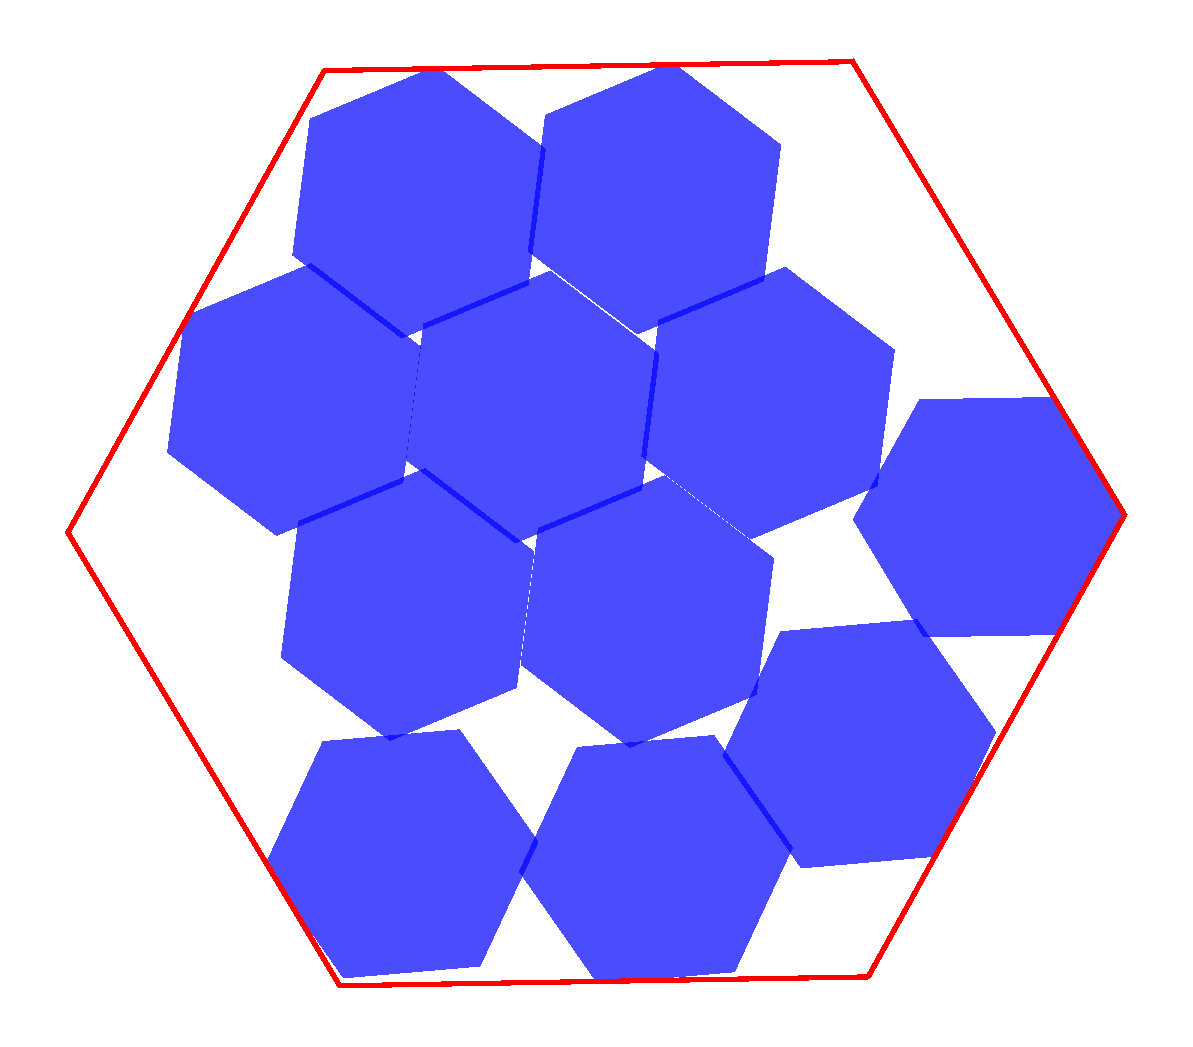
\includegraphics[width=0.4\linewidth]{figures/hexagon_11.pdf}
    \hfill
    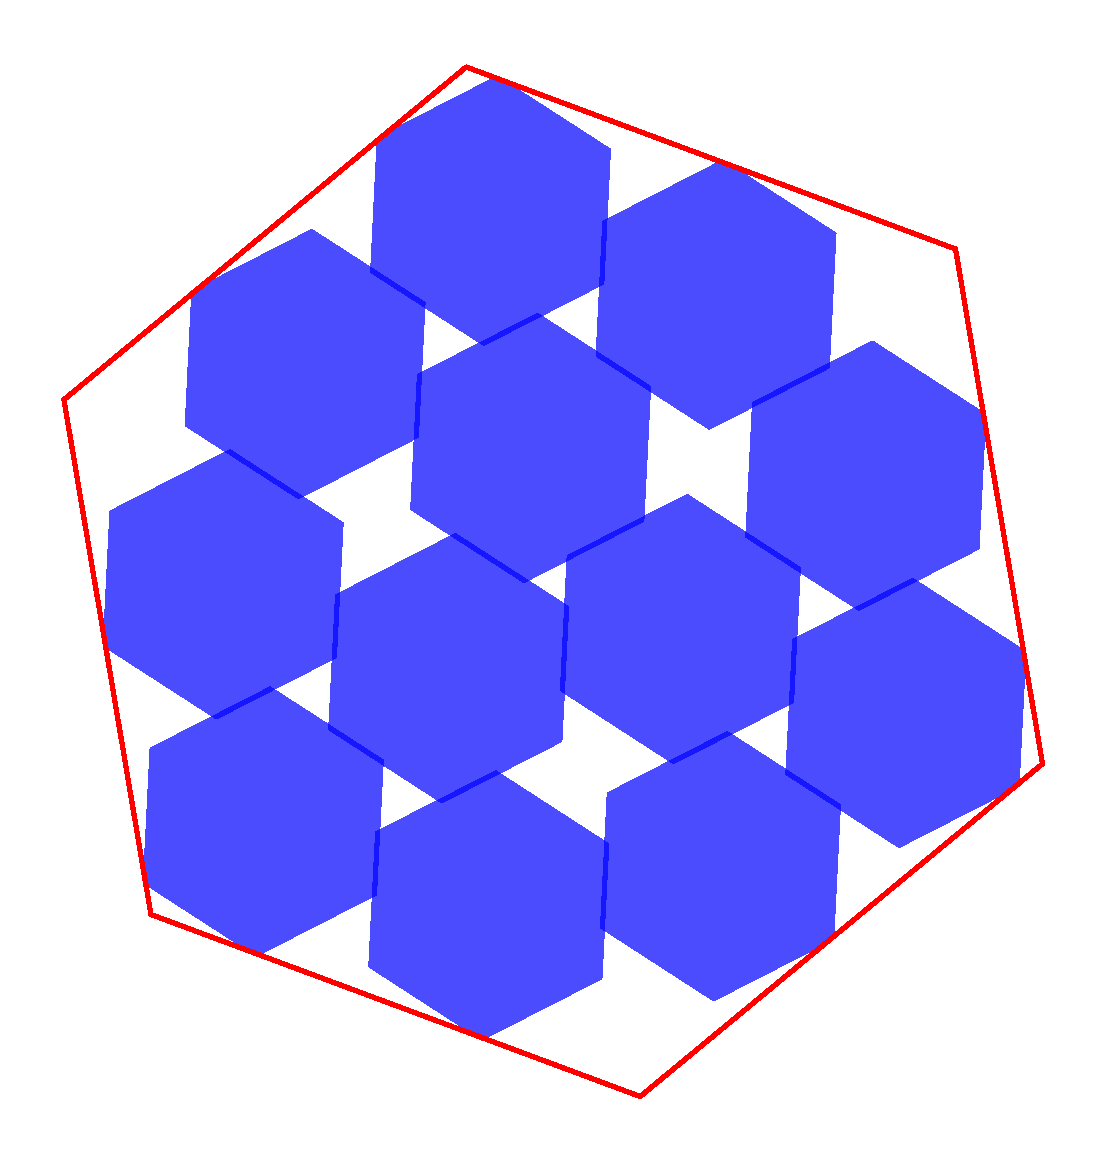
\includegraphics[width=0.4\linewidth]{figures/hexagon_12.pdf}
    \caption{Constructions of the packing problems found by \method. Left: Packing 11 unit hexagons into a regular hexagon of side length 3.931. Right: Packing 12 unit hexagons into a regular hexagon of side length 3.942.
    \label{fig:hexagons}}
\end{figure}


\subsection{Minimizing the ratio of maximum to minimum distance}
For any $n$ and $d$, the goal of this problem is to find $n$ points in the $d$-dimensional space so as to minimize the ratio between the maximum and minimum pairwise distances. \method found two new constructions improving the best known bounds.
The found constructions are shown in \Cref{fig:distance_ratios}.

In 2 dimensions, \method found 16 points with ratio $\approx \sqrt{12.889266112}$, improving the best known bound of $\sqrt{12.890}$~\citep{geometry_collection}.
(In this reference, instead of the ratio itself, the square of the ratio is reported, and we use the same convention.)
 
In 3 dimensions, \method found 14 points with ratio $\approx \sqrt{4.165849767}$, improving the best known bound of $\sqrt{4.168}$~\citep{geometry_collection}.

\begin{figure}
    \centering
    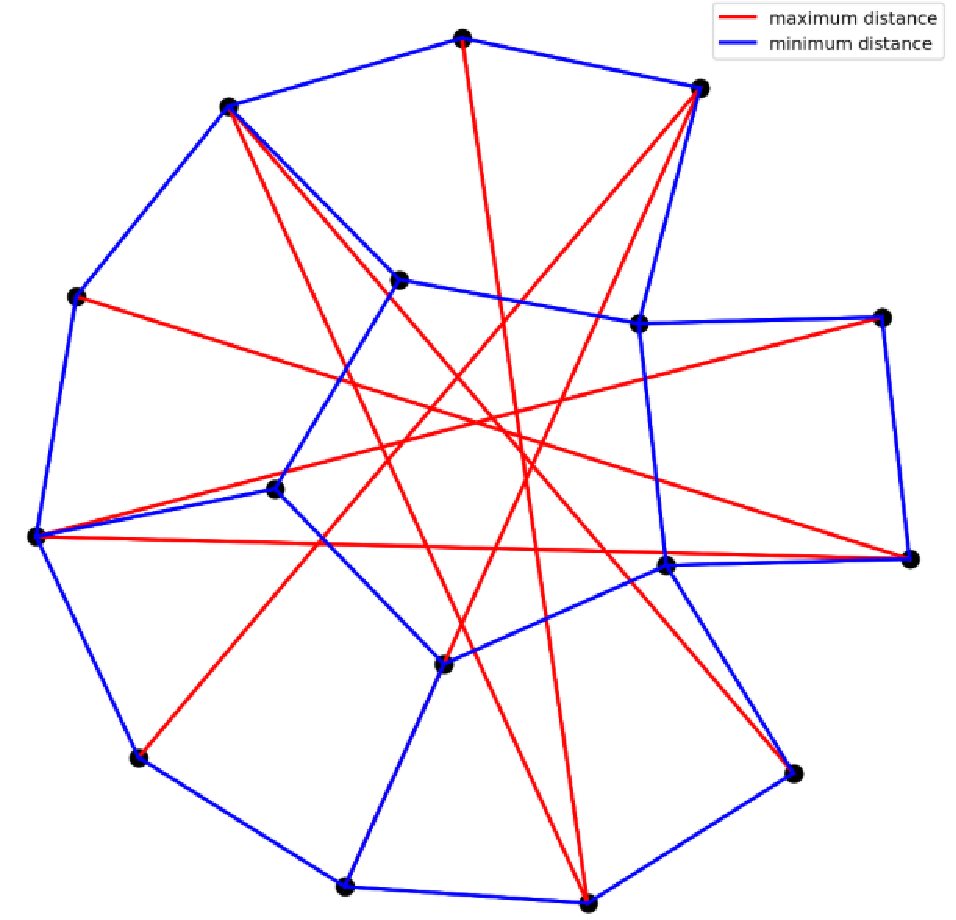
\includegraphics[width=0.45\linewidth]{figures/maxmin1.pdf}
    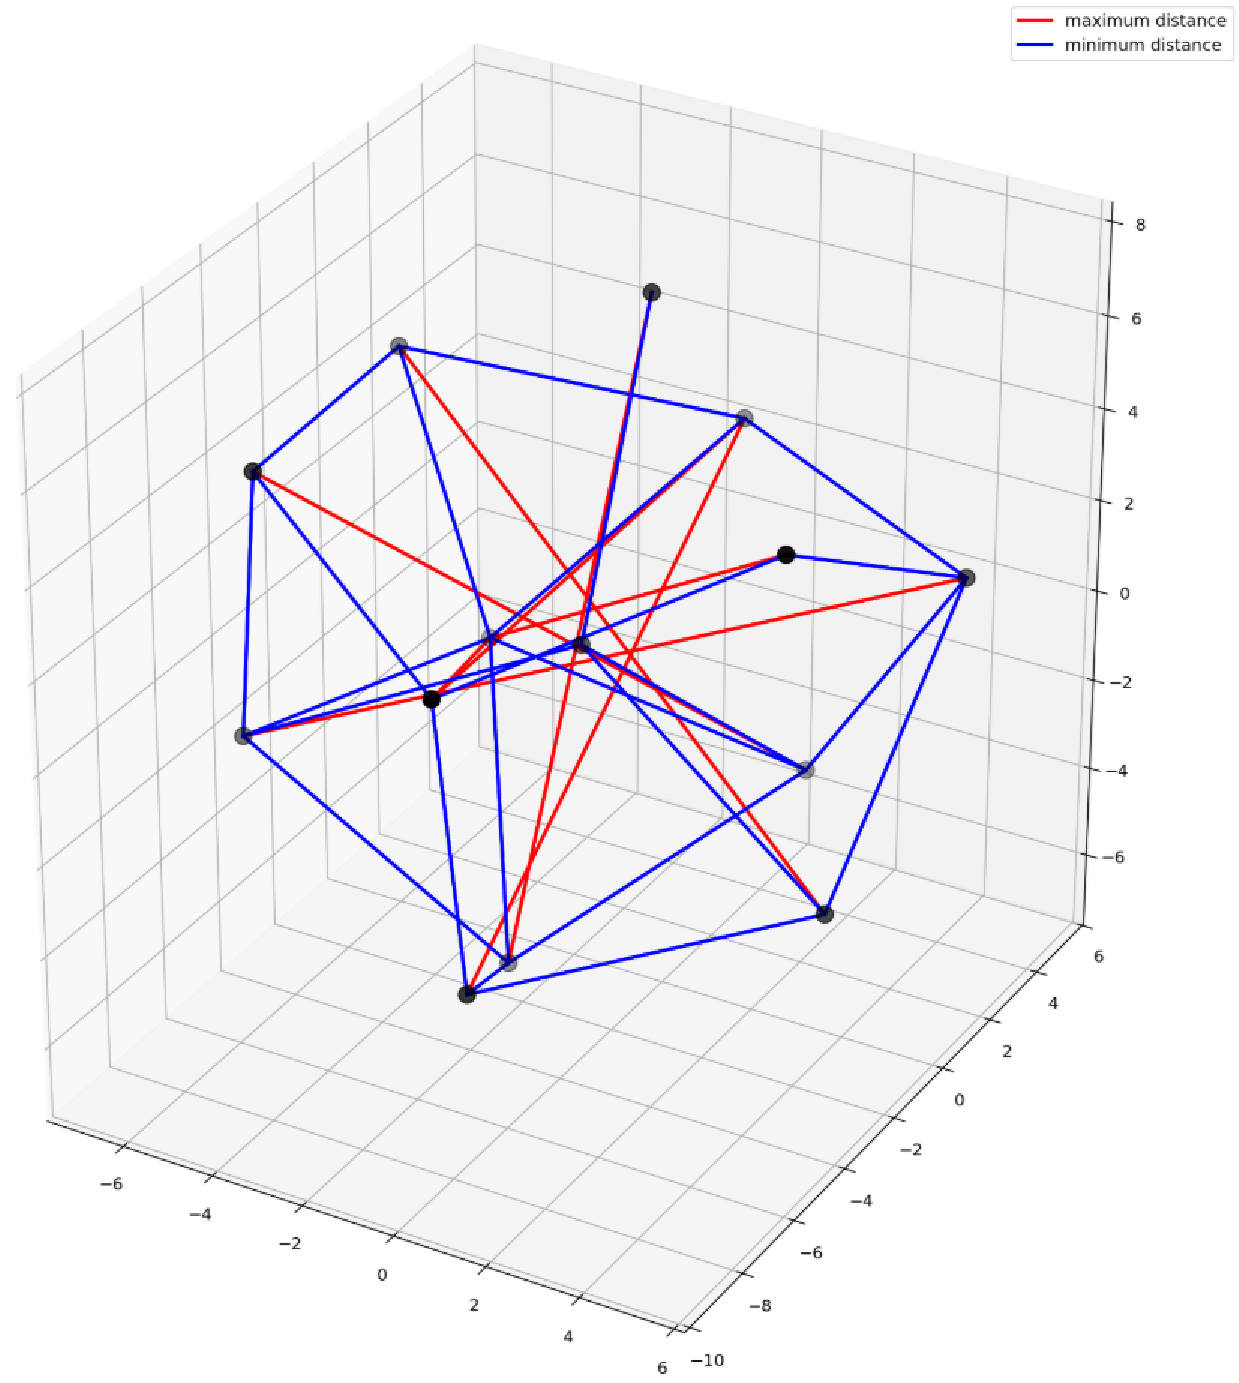
\includegraphics[width=0.45\linewidth]{figures/maxmin2.pdf}
    \caption{Left: 16 points in 2 dimensions achieving a ratio of maximum distance to minimum distance of
    $\approx \sqrt{12.889266112}$.     
    Right: 14 points in 3 dimensions achieving a ratio of $\approx \sqrt{4.165849767}$. Both constructions improve the best known bounds.}
    \label{fig:distance_ratios}
\end{figure}


\subsection{The Heilbronn problem for triangles}
The goal of this problem is to find $n$ points on or inside a triangle with unit area so that the area of the smallest triangle formed by these points is maximized. For $n=11$, the SOTA was $0.036$~\citep{geometry_collection}, and AlphaEvolve found a construction with minimum area larger than $0.0365$, which is shown in \Cref{fig:heilbronn} (left). 

\subsection{The Heilbronn problem for convex regions}
The goal of this problem is to find $n$ points on or inside a convex region with unit area so that the area of the smallest triangle formed by these points is maximized. \method improved two of the best known bounds.

For $n=13$, the SOTA was $0.0306$~\citep{geometry_collection}, and \method improved it to $0.0309$ (see \Cref{fig:heilbronn} (middle)).
For $n=14$, the SOTA was $0.0277$~\citep{geometry_collection} and \method improved it to $0.0278$ (see \Cref{fig:heilbronn} (right)).

\begin{figure}
    \centering
    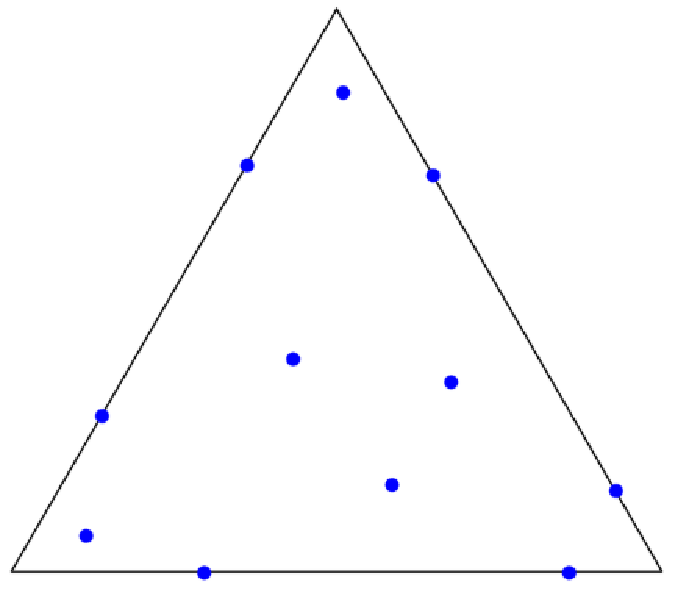
\includegraphics[width=0.25\linewidth]{figures/Heilbronn_triangle.pdf}
    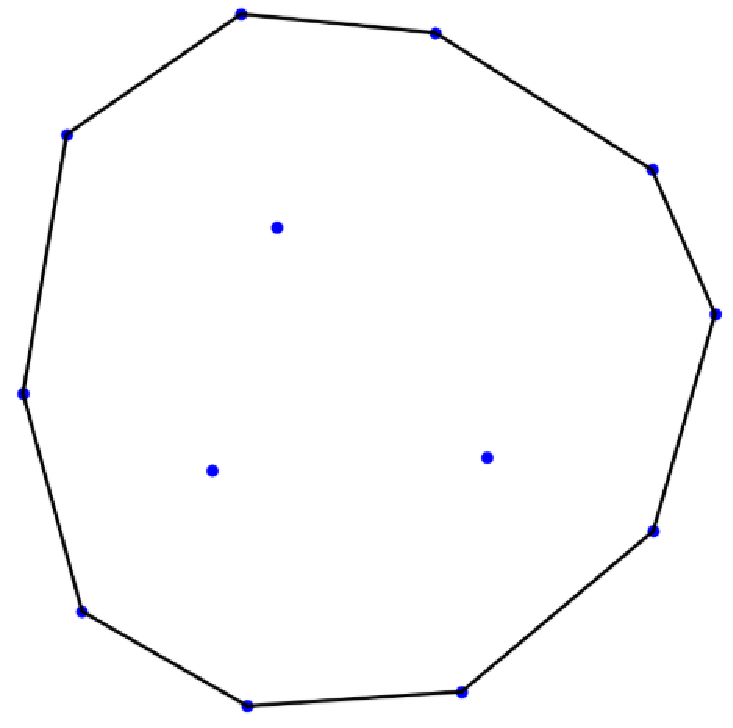
\includegraphics[width=0.25\linewidth]{figures/Heilbronn_convex_1.pdf}
    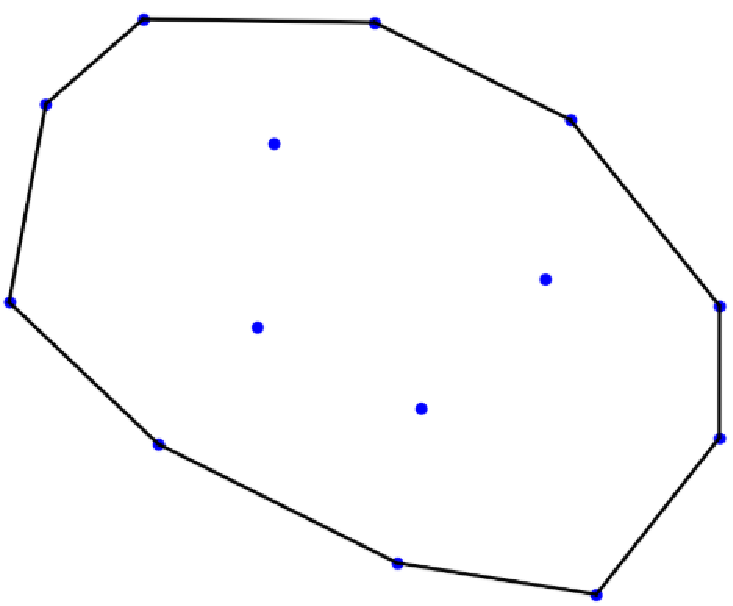
\includegraphics[width=0.25\linewidth]{figures/Heilbronn_convex_2.pdf}
    \caption{New constructions found by \method improving the best known bounds on two variants of the Heilbronn problem. Left: 11 points in a unit-area triangle with all formed triangles having area $\geq 0.0365$. Middle: 13 points inside a convex region with unit area with all formed triangles having area $\geq 0.0309$. Right: 14 points inside a unit convex region with minimum area  $\ge 0.0278$.}
    \label{fig:heilbronn}
\end{figure}


\subsection{Kissing number in dimension 11}
The kissing problem asks how many disjoint unit spheres can be packed tangent to a given unit sphere. The maximum such number in $d$ dimensions is called the \emph{$d$-dimensional kissing number~\citep{kissing_survey}}.
For $d=11$, the best known lower bound was 592~\citep{kissing_11} and \method improved this to 593. To prove the lower bound of 593 for the kissing number in dimension 11, \method found 593 many 11-dimensional non-zero points with integral coordinates such that  
the maximum norm of these points is smaller than their minimum pairwise distance.
By the following lemma, this implies the kissing number in dimension 11 is at least 593.

\begin{lemma}
Let $C \subset \mathbb{R}^d$ be a set of points satisfying
$0 \notin C$ and 
\begin{equation*}
    \min \left\{ \|x-y\| : x \neq y \in C \right\} \ge \max \left\{ \|x\|: x \in C \right\}.
\end{equation*}
Then unit spheres centred at $\left\{  \frac{2x}{\|x\|}:{x\in C}\right\}$ form a valid kissing configuration in dimension $d$. In particular, the kissing number in dimension $d$ is at least $|C|$.
\end{lemma}

\begin{proof}
For any $x\neq y \in C$, the inequality $\|x - y\|^2 \geq \max \{\|x\|^2, \|y\|^2\}$ implies
\begin{equation}
2 \langle x, y \rangle \leq \|x\|^2 + \|y\|^2 - \max \{\|x\|^2, \|y\|^2\} = \min \{\|x\|^2, \|y\|^2\} \leq \|x\|\cdot\|y\|,
\label{eq:abi}
\end{equation}
where the last inequality holds because the minimum of two positive numbers is less than or equal to their geometric mean.
The points $\left\{ \frac{2x}{\|x\|}:{x\in C}\right\}$ have norm 2, so unit spheres centred at them are tangent to a unit sphere centred at the origin.
The last step is to show that these spheres do not overlap. This is equivalent to showing, for all $x\neq y \in C$, that
\[
\left\| \frac{2x}{\|x\|} -  \frac{2y}{\|y\|}\right\| \geq 2.
\]
After simplifying, this is equivalent to
\(
2 \langle x, y \rangle  \leq \|x\|\cdot\|y\|\),
which we have proved in \eqref{eq:abi}.
Thus unit spheres centred at $\left\{ \frac{2x}{\|x\|}:{x\in C}\right\}$ form a valid kissing configuration in dimension $d$, as required.
\end{proof}


\subsection{Packing circles inside a unit square to maximize sum of radii}

Given a positive integer $n$, the problem is to pack $n$ disjoint circles inside a unit square so as to maximize the sum of their radii. \method found two new constructions improving the state of the art~\citep{geometry_collection}.

For $n=26$, the SOTA was $2.634$, and AlphaEvolve improved it to $2.635$; see \Cref{fig:circle_packing} (left).
For $n=32$, the SOTA was $2.936$, and AlphaEvolve improved it to $2.937$; see \Cref{fig:circle_packing} (middle).

\subsection{Packing  circles inside a rectangle of perimeter 4 to maximize sum of radii}
Given a positive integer $n$, the problem is to pack $n$ disjoint circles inside a rectangle of perimeter 4 so as to maximize the sum of their radii. 
\method found a new construction for $n=21$, improving the state of the art from $2.364$~\citep{geometry_collection} to $2.3658$; see \Cref{fig:circle_packing} (right).

\begin{figure}[b]
    \centering
    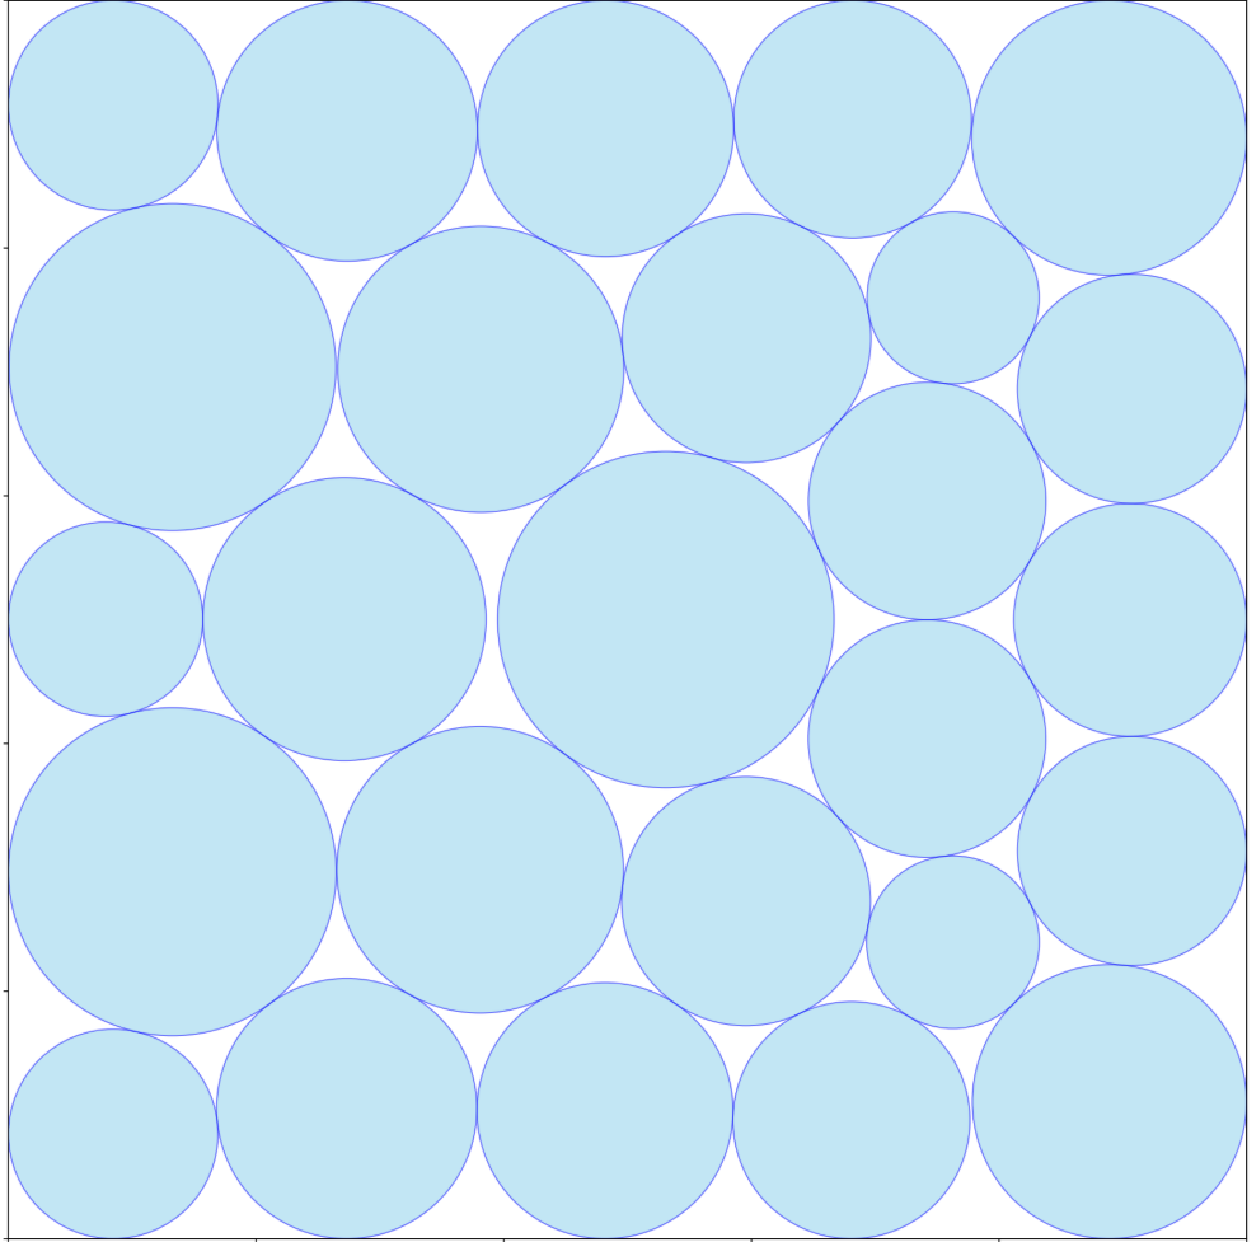
\includegraphics[width=0.25\linewidth]{figures/circles_1.pdf}
    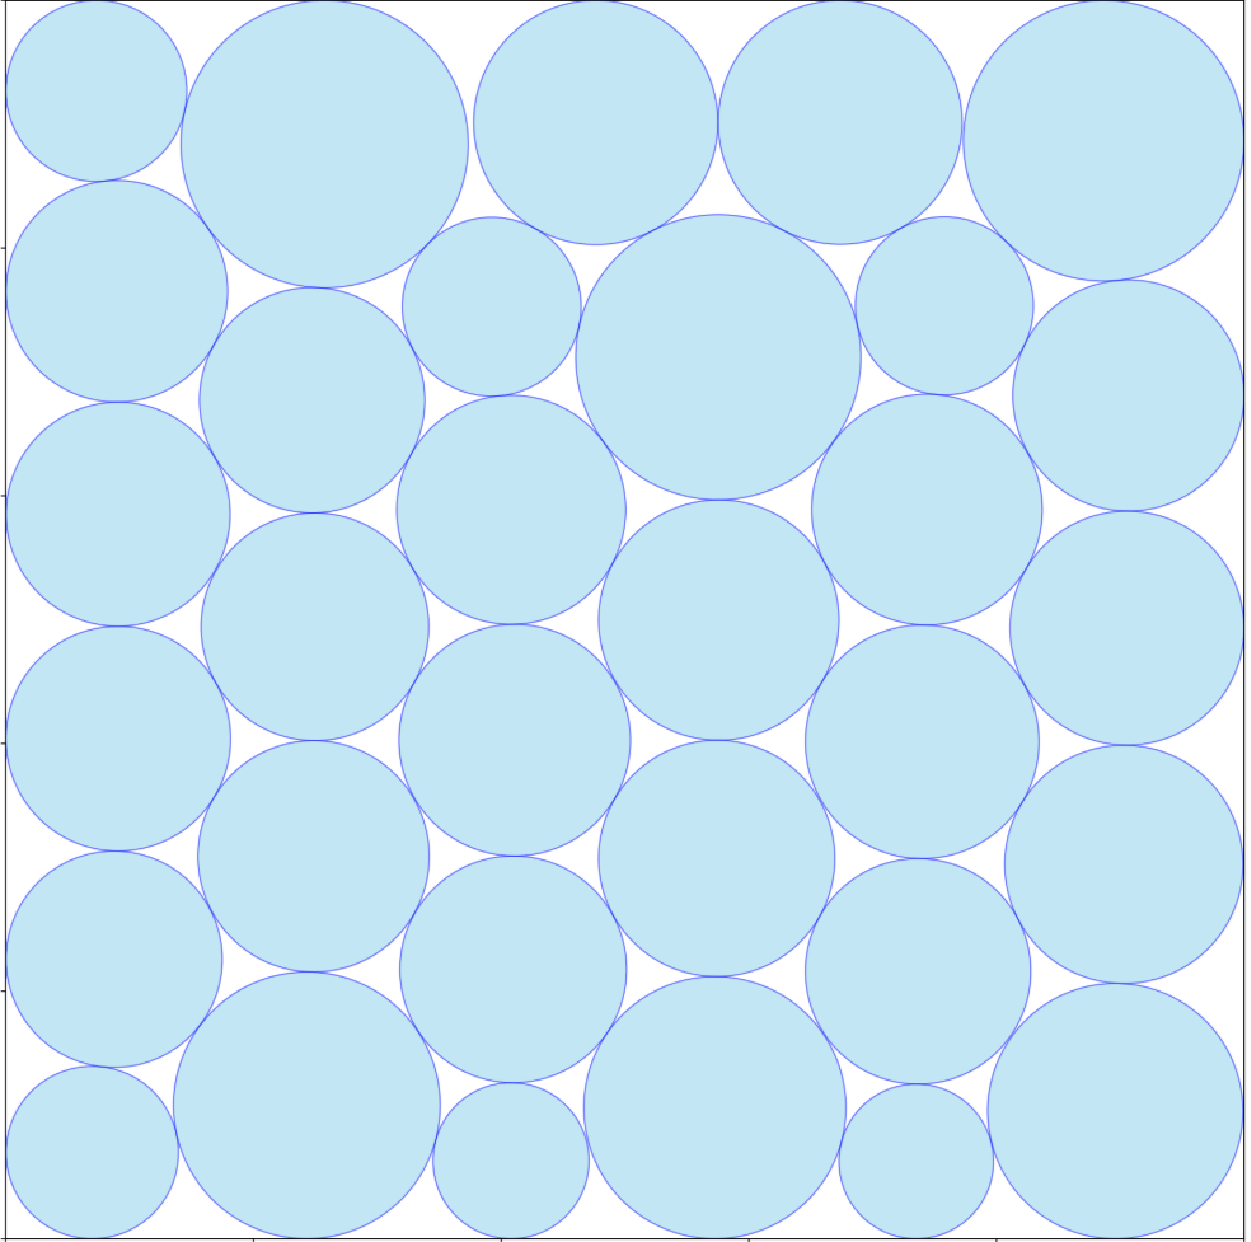
\includegraphics[width=0.25\linewidth]{figures/circles_2.pdf}
    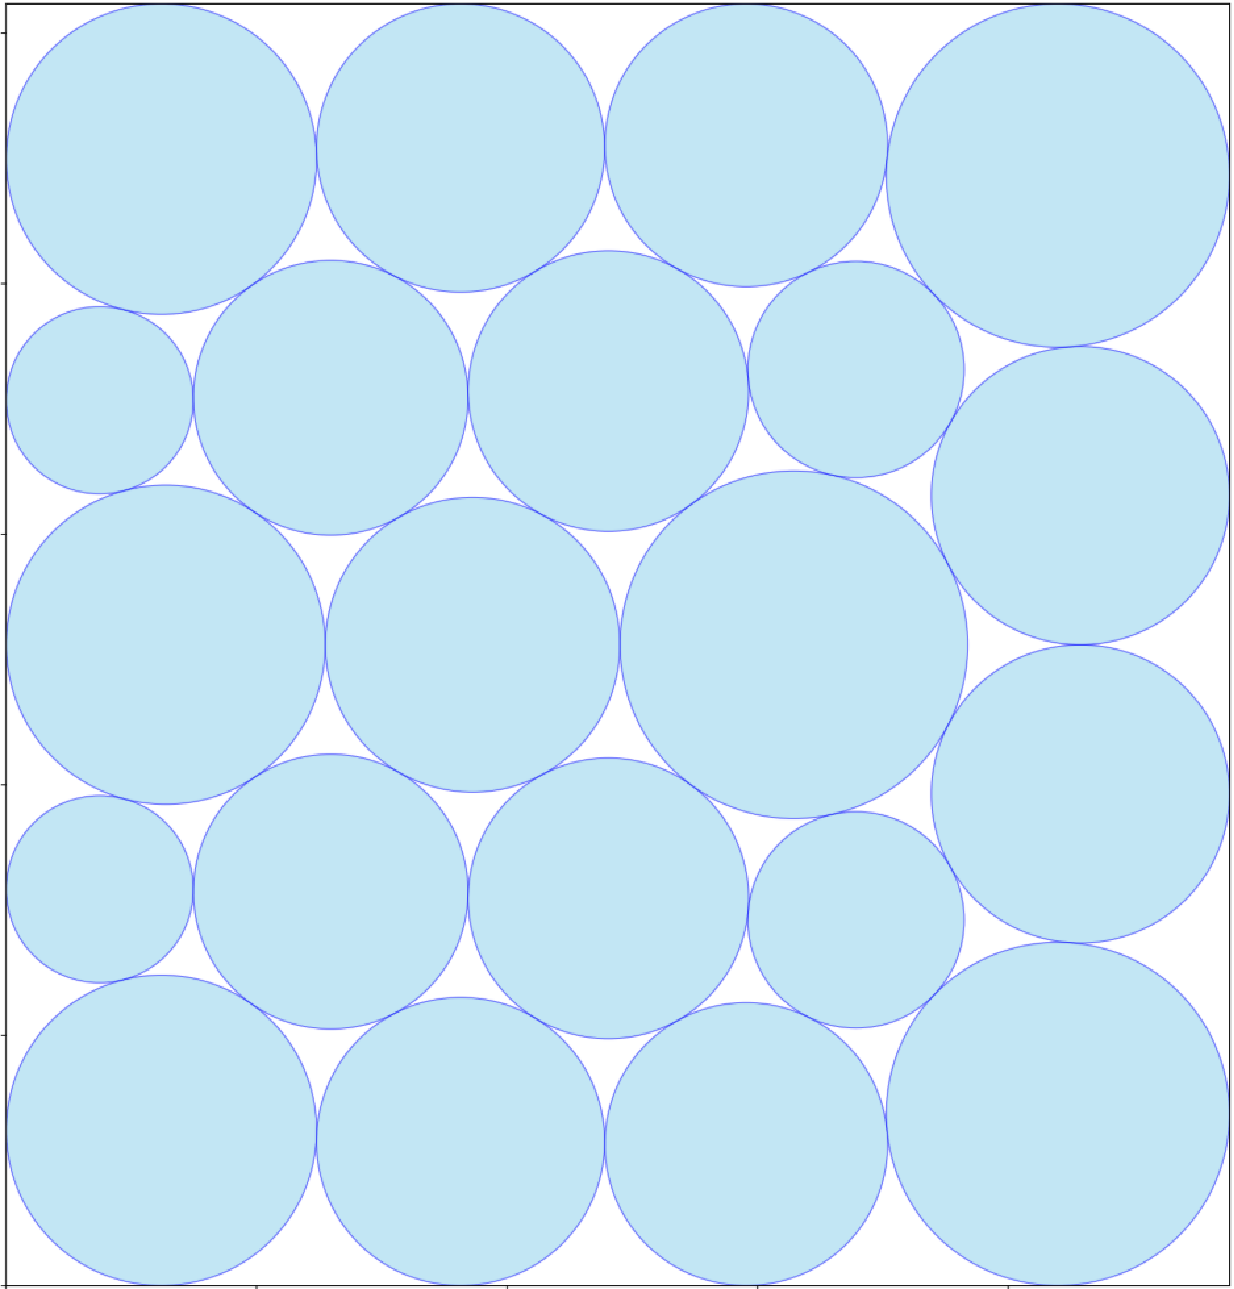
\includegraphics[width=0.25\linewidth]{figures/circles_3.pdf}
    \caption{New constructions found by \method improving the best known bounds on packing circles to maximize their sum of radii. Left: $26$ circles in a unit square with sum of radii $\geq 2.635$. Middle: $32$ circles in a unit square with sum of radii $\geq 2.937$. Right: 21 circles in a rectangle with perimeter $4$, with sum of radii $\geq 2.365$.}
    \label{fig:circle_packing}
\end{figure}

\section{Proof of Lemma 3.1}

\paragraph{Proof.} 

Let $\mathcal{I}^{=0}(\bm{x}):=\{i| \bm{x}_i=0\}$ be the set of indices of zero elements at $\bm{x}$. The output deviation between the original network output and the gated output via a general-format sparsification is:

\begin{align*}
	\norm{W(\bm{x}_{\mathcal{I}^{=0}} - \bm{x})}^2 &= \left\| \sum_{i\in \mathcal{I}^{=0}} \bm{x}_i W_{:,i} \right\|_2^2 \\
	&= \left( \sum_{i\in \mathcal{I}^{=0}} x_i W_{:,i} \right)^{\top} \left( \sum_{i\in \mathcal{I}^{=0}} \bm{x}_i W_{:,i} \right) \\
	&= \sum_{j \in  \mathcal{I}^{=0}} \sum_{i \in  \mathcal{I}^{=0}} \bm{x}_j \bm{x}_i W_{:,j}^\top W_{:,i} \\
	&= \sum_{i \in  \mathcal{I}^{=0}} \bm{x}_i^2 \| W_{:,i} \|_2^2 + \sum_{i\neq j  \in  \mathcal{I}^{=0}} \bm{x}_j \bm{x}_i W_{:,j}^\top W_{:,i}
\end{align*}

The expected output deviation for \algacro{} is:

% \begin{align}\label{equ}
	% e_{\text{TEAL}} &= \E{\norm{Wx_{\text{TEAL}} - Wx }^2} \\
	% &= \sum_{j \in  Z_{\text{TEAL}}} \mathbb{E}[x_j^2 \| W_{:,j} \|_2^2] + \sum_{i \neq j \in  Z_{\text{TEAL}}} \mathbb{E}[x_j x_i W_{:,j}^T W_{:,i}]
	% \end{align}

% Similarly, the expected output deviation for \algacro{} sparsification is:

\begin{align*}
	e_{\text{\algacro{}}} &= \norm{W\bm{x}_{\mathcal{I}^{=0}_{\text{\algacro{}}}} - W\bm{x}}^2 \\
	&= \sum_{i \in \mathcal{I}^{=0}_{\text{\algacro{}}}} \bm{x}_i^2 \| W_{:,i} \|_2^2 + \sum_{i \neq j \in \mathcal{I}^{=0}_{\text{\algacro{}}}} \bm{x}_j \bm{x}_i W_{:,j}^\top W_{:,i}.
\end{align*}

Since $W$ is assumed to be column orthogonal, the cross-term expectations vanish, and the expected output error is determined solely by the main term:
$$
e_{\text{\algacro{}}} = \sum_{i \in \mathcal{I}^{=0}_{\text{\algacro{}}}} \bm{x}_i^2 \| W_{:,i} \|_2^2.
$$

Because \algacro{} sparsification sets the $k$ smallest $|\bm{x}_i\bm{c}_i|$ terms to zero, we have the mask of \algacro{} reaches out the lower bound of approximation error for a single layer network, \ie,
\begin{equation}
	\bm{g}_{\text{\algacro{}}}(\bm{x})=\argmin_{\bm{g}\in\{0,1\}^{n}}\quad \norm{W(\bm{x}\odot \bm{g} - \bm{x})}^2.
\end{equation}

Thus, the above indicates that \algacro{} sparsification achieves the tight lower bound of the approximation error, including those of TEAL and CATS. 
\section{Proof of Theorem 3.2}

\paragraph{Proof.} We prove this by mathematical induction. 
\paragraph{Step 1: Base case $N=2$.} The output error for sparse activation parameterized via mask $\bm{g}$ is:
\begin{align*}\label{equ}
	&\norm{\bm{y}_{\bm{g}}^{(2)} - \bm{y}^{(2)}} \\
	= &\norm{W^{(2)} (\bm{y}_{\bm{g}}^{(1)} \odot \bm{g}^{(2)}) - W^{(2)} \bm{y}^{(1)}} \\
	= &\norm{W^{(2)} (\bm{y}_{\bm{g}}^{(1)} \odot \bm{g}^{(2)}) - W^{(2)}\bm{y}_{\bm{g}}^{(1)} + W^{(2)}\bm{y}_{\bm{g}}^{(1)}-W^{(2)} \bm{y}^{(1)}} \\
	= &\norm{W^{(2)}{(\bm{y}_{\bm{g}}^{(1)} \odot \bm{g}^{(2)} - \bm{y}_{\bm{g}}^{(1)})} + W^{(2)}{(\bm{y}_{\bm{g}}^{(1)} - \bm{y}^{(1)})}}\\
	= &\norm{W^{(2)}{(\bm{y}_{\bm{g}}^{(1)} \odot \bm{g}^{(2)} - \bm{y}_{\bm{g}}^{(1)}}) + W^{(2)}(W^{(1)} \bm{x}\odot \bm{g}^{(1)} - W^{(1)} \bm{x})}
\end{align*}
Let: 
$$
\Delta^{(1)} = \text{diag}(\bm{g}^{(1)} - 1),\quad \Delta^{(2)} = \text{diag}(\bm{g}^{(2)} - 1), \quad M^{(1)} = \text{diag}(\bm{g}^{(1)}).
$$
Then, let $\bm{v}$ and $\bm{u}$ be 
\begin{align*}
	\bm{v} &=W^{(2)}(\bm{y}_{\bm{g}}^{(1)}\odot(\bm{g}^{(2)}-{1}))\\
	&=W^{(2)}(W^{(1)}(\bm{x}\odot \bm{g}^{(1)})\odot(\bm{g}^{(2)}-1)) \\
	&=W^{(2)}\Delta^{(2)}W^{(1)}M^{(1)}\bm{x}\\
	\bm{u} &=W^{(2)}W^{(1)}(\bm{x}\odot(\bm{g}^{(1)}-1))\\
	&=W^{(2)}W^{(1)}\Delta^{(1)}\bm{x}. \\
\end{align*}
Since $\E{\norm{\bm{u} + \bm{v}}^2} = \E{\norm{\bm{u}}^2} + \E{\norm{\bm{v}}^2} + 2\E{(\bm{u}^\top\bm{v})}$, the expected value of the cross-term is:
\begin{align*}
	\E[\bm{u}^\top\bm{v}] &= \E[\bm{x}^\top\Delta^{(1)}(W^{(1)})^\top(W^{(2)})^\top(W^{(2)})\Delta^{(2)}W^{(1)}M^{(1)}\bm{x}] \\
	&= \E[\text{tr}(W^{(2)}\Delta^{(2)}W^{(1)}M^{(1)}\bm{x}\bm{x}^\top\Delta^{(1)}(W^{(1)})^\top(W^{(2)})^\top)] \\
	&= \text{tr}\left(W^{(2)}\E[\Delta^{(2)}]W^{(1)}\E[M^{(1)}\Delta^{(1)}]\E[\bm{x}\bm{x}^\top](W^{(1)})^\top(W^{(2)})^\top\right)
\end{align*} 
Since $\E[M_1\Delta_1]=\E[\bm{g}^{(1)}\odot(\bm{g}^{(1)}-1)]=0$, the cross-term expectation $\E[\bm{u}^\top\bm{v}]$ is zero. Thus, the expected output deviation via sparse activation $\bm{g}$,
\begin{equation}
	\begin{split}
		e^{(2)}&=\E[\norm{\bm{u}+\bm{v}}^2]\\    
		&=\E[\norm{W^{(2)}{(\bm{y}_{\bm{g}}^{(1)} \odot \bm{g}^{(2)} - \bm{y}_{\bm{g}}^{(1)}})}^2] +\E[\norm{W^{(2)}(W^{(1)} \bm{x}\odot \bm{g}^{(1)} - W^{(1)} \bm{x})}^2]
	\end{split}
\end{equation}
Upon Lemma~\ref{lemma.single_layer}, we have that
$$
\mathbb{E}[\| W^{(2)}(W^{(1)} \bm{x}\odot \bm{g}_{\text{\algacro{}}}^{(1)} - W^{(1)} \bm{x}) \|^2] \leq \mathbb{E}[\| W^{(2)}(W^{(1)} \bm{x}\odot \bm{g}_{\text{TEAL}}^{(1)} - W^{(1)} \bm{x}) \|^2]
$$
Next, we compare $\mathbb{E}[\|W^{(2)}(\bm{y}_{\bm{g}}^{(1)} \odot \bm{g}^{(2)} - \bm{y}_{\bm{g}}^{(1)})\|^2]$ given $\bm{g}_\text{\algacro{}}^{(2)}$ and $\bm{g}_\text{TEAL}^{(2)}$.
\begin{align*}
	&\ \mathbb{E}[\|W^{(2)}(\bm{y}_{\bm{g}}^{(1)} \odot \bm{g}^{(2)} - \bm{y}_{\bm{g}}^{(1)})\|^2]\\
	=&\ \E[{\sum_{j\in \mathcal{I}^{=0}(\bm{g}^{(2)})}\sum_{i\in \mathcal{I}^{=0}(\bm{g}^{(2)})} \bm{y}_j^{(1)}\bm{y}_i^{(1)}\,(W_{:,j}^{(2)})^\top W_{:,i}^{(2)}}]\\
	= &\E[{\sum_{j\in \mathcal{I}^{=0}(\bm{g}^{(2)})} (\bm{y}_j^{(1)})^2\|W_{:,j}^{(2)}\|^2 + \sum_{\substack{i,j\in \mathcal{I}^{=0}(\bm{g}^{(2)})\\i\neq j}} \bm{y}_j^{(1)}\bm{y}_i^{(1)}\,(W_{:,j}^{(2)})^T W_{:,i}^{(2)}}]\\
	= &\ \sum_{j\in \mathcal{I}^{=0}(\bm{g}^{(2)})}{(\bm{c}_j^{(2)})^2\E{(\bm{y}_{j}^{(1)})^2}} + \sum_{\substack{i,j\in \mathcal{I}^{=0}(\bm{g}^{(2)})\\i\neq j}}({W_{:,j}^{(2)})^\top W_{:,i}^{(2)}\E[{\bm{y}_j^{(1)}\bm{y}_i^{(1)}}]}\\
	= &\ \sum_{j\in \mathcal{I}^{=0}(\bm{g}^{(2)})}{(\bm{c}_j^{(2)})^2\E{(\bm{y}_{j}^{(1)})^2}},
\end{align*}
where the last line is due to $W^{(2)}$ is column-orthogonal, the cross-term's expectation is zero.

Because \algacro{} sparsification sets the $k$ smallest $(\bm{y}_j^{(1)}c_j^{(2)})^2$ terms to zero, we have:
$$
\mathbb{E}[\|W^{(2)}(\bm{y}_{\bm{g}_\text{\algacro{}}}^{(1)} \odot \bm{g}^{(2)} - \bm{y}_{\bm{g}_\text{\algacro{}}}^{(1)})\|^2]\leq \mathbb{E}[\|W^{(2)}(\bm{y}_{\bm{g}_\text{TEAL}}^{(1)} \odot \bm{g}^{(2)} - \bm{y}_{\bm{g}_{\text{TEAL}}}^{(1)})\|^2]
$$
Therefore, we have that 
$$
e_{\text{\algacro{}}}^{(2)}\leq e_{\text{TEAL}}^{(2)}.
$$
\paragraph{Step 2: Inductive proof for $N>2$.}
Assume for some $N\ge2$ that
$$
e_{\text{\algacro{}}}^{(N)}\leq e_{\text{TEAL}}^{(N)}.
$$
Define the exact output of $(N+1)$ layer network:
$$
\bm{y} = W^{(N+1)} \bm{y}^{(N)}, \quad \bm{y}^{(N)} = W^{(N)}\cdots W^{(1)}\bm{x}
$$
The output via mask $\bm{g}^{(N+1)}$ is that
\begin{align*}
	&\ \bm{y}_{\bm{g}}^{(N+1)} - \bm{y} \\
	=\ &\ W^{(N+1)}(\bm{y}_{\bm{g}}^{(N)} \odot \bm{g}^{(N+1)}) - W^{(N+1)}\bm{y}^{(N)} \\
	=\ &\ W^{(N+1)}((\bm{y}_{\bm{g}}^{(N)} \odot \bm{g}^{(N+1)} ) - \bm{y}_{\bm{g}}^{(N)}) + W^{(N+1)}(\bm{y}_{\bm{g}}^{(N)} - \bm{y}^{(N)})
\end{align*}
The expected output deviation is:
\begin{equation}
	e_{\bm{g}}^{N+1}=\E\|W^{(N+1)}(\bm{y}_{\bm{g}}^{(N)} \odot \bm{g}^{(N+1)} - \bm{y}_{\bm{g}}^{(N)})\|^2 + \E\|W^{(N+1)}(\bm{y}_{\bm{g}}^{(N)} - \bm{y}^{(N)})\|^2,
\end{equation}
the cross-term zeros out because of the assumption. 

Upon induction assumption, for the second term, we have that 
\begin{equation}
	\E\|W^{(N+1)}(\bm{y}_{\bm{g}_\text{\algacro{}}}^{(N)} - \bm{y}^{(N)})\|^2\leq \E\|W^{(N+1)}(\bm{y}_{\bm{g}_\text{TEAL}}^{(N)} - \bm{y}^{(N)})\|^2.
\end{equation}
For the first term, we have that 
\begin{align*}
	&\ \mathbb{E}[\|W^{(N+1)}(\bm{y}_{\bm{g}}^{(N)} \odot \bm{g}^{(N+1)} - \bm{y}_{\bm{g}}^{(N)})\|^2]\\
	=&\ \E[{\sum_{j\in \mathcal{I}^{=0}(\bm{g}^{(N+1)})}\sum_{i\in \mathcal{I}^{=0}(\bm{g}^{(N+1)})} \bm{y}_j^{(N)}\bm{y}_i^{(N)}\,(W_{:,j}^{(N+1)})^\top W_{:,i}^{(N+1)}}]\\
	= &\ \sum_{j\in \mathcal{I}^{=0}(\bm{g}^{(N+1)})}{(\bm{c}_j^{(N+1)})^2\E{(\bm{y}_{j}^{(N)})^2}} + \sum_{\substack{i,j\in \mathcal{I}^{=0}(\bm{g}^{(N+1)})\\i\neq j}}({W_{:,j}^{(N+1)})^\top W_{:,i}^{(N+1)}\E[{\bm{y}_j^{(N)}\bm{y}_i^{(N)}}]}\\
	= &\ \sum_{j\in \mathcal{I}^{=0}(\bm{g}^{(N+1)})}{(\bm{c}_j^{(N+1)})^2\E{(\bm{y}_{j}^{(N)})^2}},
\end{align*}
where the last line is due to $W^{(N+1)}$ is column-orthogonal, the cross-term's expectation is zero.

Since \algacro{} retains the $k$ largest $|\bm{y}_j^{(N)}\bm{c}_j^{N+1}|$, thus:
\begin{equation}
	\mathbb{E}[\|W^{(N+1)}(\bm{y}_{\bm{g}}^{(N)} \odot \bm{g}_\text{\algacro{}}^{(N+1)} - \bm{y}_{\bm{g}}^{(N)})\|^2]\leq \mathbb{E}[\|W^{(N+1)}(\bm{y}_{\bm{g}}^{(N)} \odot \bm{g}_\text{TEAL}^{(N+1)} - \bm{y}_{\bm{g}}^{(N)})\|^2].
\end{equation}
Consequently, we reach the conclusion that
\begin{align}
	e_\text{\algacro{}}^{(N+1)}\leq e_\text{TEAL}^{(N+1)}.
\end{align}



\section{Proof of Lemma 3.4}

\paragraph{Proof.} 
Let $\Delta$ be the error term of the output via sparse activation parameterized with $\bm{g}$, 
$$
\Delta_{\bm{g}} = W(\bm{x} \odot (1 - \bm{g})) = \sum_{i=1}^{d} W_{i,:} \bm{x}_i \odot(1 - \bm{g}_{i}).
$$
Using a Taylor expansion and ignoring higher-order terms (assuming $ \Delta_{i}$ is small), the output deviation given an activation function $f$ is:
$$
f(W_{i,:}\bm{x} + \Delta_{\bm{g},i}) - f(W_{i,:}\bm{x}) \approx \Grad^\top f(W_{:,i}\bm{x}) \Delta_i.
$$
Thus, the expected squared output deviation between the original output and the gated output approximates to:
\begin{align*}
	e_{\bm{g}}&=\E{\left\|f(W\bm{x} + \Delta_{\bm{g}}) - f(W\bm{x})\right\|^2} \\
	&= \E{\|\sum_{i=1}^d f(W_{i,:}\bm{x} + \Delta_{\bm{g},i}) - f(W_{i,:}\bm{x})\|^2} \\
	&\approx \mathbb{E}\left[\|\sum_{i=1}^d \Grad f(W_{i,:}\bm{x})\Delta_{\bm{g}, i}\|^2\right]\\
	&= \sum_{i=1}^d \E [\Grad^2 f(W_{i,:}\bm{x})\Delta_{\bm{g}, i}^2]\\
	&=\sum_{i=1}^d \E [\Grad^2 f(W_{i,:}\bm{x})(W_{i,:} \bm{x}_i\odot (1 - \bm{g}_{i}))^2]\\
	&=\sum_{i=1}^d \E [\Grad^2 f(W_{i,:}\bm{x})] \sum_{i=1}^d\E (W_{i,:} \bm{x}_i\odot (1 - \bm{g}_{i}))^2\\
	&=\sum_{i=1}^d \E [\Grad^2 f(W_{i,:}\bm{x})] \sum_{i\in \mathcal{I}^{=0}(\bm{g})}^d\E[\bm{c}_i^2 \bm{x}_i^2]
\end{align*}
Because \algacro{} sparsification select the $k$ smallest $\bm{x}_j^2 \bm{c}_j^2$ terms to zero, we have that
\begin{align}
	e_\text{\algacro{}}\leq e_\text{TEAL}.
\end{align}

\section{Proof of Theorem 3.5}

\paragraph{Proof.} We prove this by mathematical induction. 
\paragraph{Step 1: Base case $N=2$.}
The output error for sparse activation via $\bm{g}^{(2)}$ is:
\begin{align*}
	&\norm{\bm{y}_{\bm{g}}^{(2)} - \bm{y}^{(2)}} \\
	= &\norm{W^{(2)} (f(\bm{y}_{\bm{g}}^{(1)} \odot \bm{g}^{(2)}) - W^{(2)} f(\bm{y}^{(1)})} \\
	= &\norm{W^{(2)} (f(\bm{y}_{\bm{g}}^{(1)}) \odot \bm{g}^{(2)}) - W^{(2)}f(y_{\bm{g}}^{(1)}) + W^{(2)}f(y_{\bm{g}}^{(1)})-W^{(2)} f(\bm{y}^{(1)})} \\
	= &\norm{W^{(2)} (f(\bm{y}_{\bm{g}}^{(1)} \odot \bm{g}^{(2)}) - f(y_{\bm{g}}^{(1)})) + W^{(2)}(f(y_{\bm{g}}^{(1)})-f(\bm{y}^{(1)}))}.
\end{align*}
Let: 
$$
M^{(1)} = \text{diag}(\bm{g}^{(1)}), \quad M^{(2)} = \text{diag}(\bm{g}^{(2)}-1).
$$
Then, let $\bm{v}$ and $\bm{u}$ be
\begin{align*}
	\bm{v} &=W^{(2)}(f(\bm{y}_{\bm{g}}^{(1)})\odot(\bm{g}^{(2)}-1)) \\
	&=W^{(2)}M^{(2)}f(W^{(1)}M^{(1)}\bm{x})\\
	\bm{u} &=W^{(2)}[f(W^{(1)}M^{(1)}\bm{x})-f(W^{(1)}\bm{x})].
\end{align*}
% Since $\E{\norm{u + v}^2} = \E{\norm{u}^2} + \E{\norm{v}^2} + \E{2u^Tv}$, 
Let $D={W^{(2)}}^\top W^{(2)}$, then the expected value of the cross-term becomes:
\begin{align*}
	\E[{\bm{u}^\top \bm{v}}] &= \E{[f(W^{(1)}M^{(1)}x)-f(W^{(1)}x)]^\top {W^{(2)}}^\top W^{(2)} M^{(2)} f(W^{(1)}M^{(1)}x)} \\
	& = \E{\left[ f(W^{(1)}M^{(1)}x) - f(W^{(1)}x) \right]^T D M^{(2)} f(W^{(1)}M^{(1)}x)} \\
	&=\E{ \sum_{i} D_{ii} \cdot (M^{(2)})_{ii} \cdot \left( f(W^{(1)}M^{(1)}\bm{x})_i - f(W^{(1)}\bm{x})_i \right)\cdot f(W^{(1)}M^{(1)}x)_i } 
\end{align*}
When $ \bm{g}^{(2)}_i = 1 $, $ (M^{(2)})_{ii} = 0 $, and the corresponding terms disappear. When $ \bm{g}^{(2)}_i = 0 $, $ (M^{(2)})_{ii} = 1 $. Therefore:
$$ E\left[ \bm{u}^\top \bm{v} \right] = E\left[ \sum_{i:\bm{g}^{(2)}_i = 0} D_{ii} \cdot \left( f(W^{(1)}M^{(1)}\bm{x})_i - f(W^{(1)}\bm{x})_i \right)\cdot  f(W^{(1)}M^{(1)}\bm{x})_i \right] $$
Since $\bm{x}$ follows a symmetric distribution with mean 0, and $W^{(1)}$ has orthogonal columns, the distributions of $W^{(1)}M^{(1)}\bm{x}$ and $W^{(1)}x$ are symmetric. For any activation function $f$, the cross-term cancels out under the symmetric distribution. Thus, the expected output deviation becomes
\begin{align*}\label{equ}
	e_{\bm{g}}^{(2)} &= \E[\norm{\bm{u}+\bm{v}}^2] =\E[\norm{\bm{u}}^2]+\E[\norm{\bm{v}}^2]\\
	&= \E[\| W^{(2)}M^{(2)}f(W^{(1)}M^{(1)}\bm{x}) \|^2] + \mathbb{E}[\| W^{(2)}[f(W^{(1)}M^{(1)}\bm{x})-f(W^{(1)}\bm{x})] \|_2^2]
\end{align*}
Here, the latter one yields the below due to Lemma~\ref{lemma:single_layer_act_function}.
$$
\mathbb{E}[\| W^{(2)}[f(W^{(1)}M_\text{\algacro{}}^{(1)}\bm{x})-f(W^{(1)}\bm{x})] \|^2] \leq \mathbb{E}[\| W^{(2)}[f(W^{(1)}M_\text{TEAL}^{(1)}\bm{x})-f(W^{(1)}\bm{x})] \|^2].
$$
Next, we compare the former term. We have that:
\begin{align*}
	&\mathbb{E}[\| W^{(2)} (f(\bm{y}_{\bm{g}}^{(1)}) \odot \bm{g}^{(2)}) - W^{(2)} f(\bm{y}_{\bm{g}}^{(1)}) \|^2] \\
	= &\E{\sum_{j\in \mathcal{I}^{=0}(\bm{g}^{(1)})}\sum_{i\in \mathcal{I}^{=0}(\bm{g}^{(1)})} f(\bm{y}_j^{(1)})\,f(\bm{y}_i^{(1)})\,(W_{:,j}^{(2)})^T W_{:,i}^{(2)}}\\
	= & \E{\sum_{j\in \mathcal{I}^{=0}(\bm{g}^{(1)})} f(\bm{y}_j^{(1)})^2\|W_{:,j}^{(2)}\|^2} 
	+ \sum_{\substack{i,j\in \mathcal{I}^{=0}(\bm{g}^{(1)})\\i\neq j}} f(\bm{y}_j^{(1)})\,f(\bm{y}_i^{(1)})(W_{:,j}^{(2)})^\top W_{:,i}^{(2)} \\
	= & \sum_{j\in \mathcal{I}^{=0}(\bm{g}^{(1)})}{(\bm{c}_j^{(2)})^2\E{f(\bm{y}_{\bm{g},j}^{(1)})^2}} + \sum_{\substack{i,j\in \mathcal{I}^{=0}(\bm{g}^{(1)})\\i\neq j}}({W_{:,j}^{(2)})^T W_{:,i}^{(2)}\E{f(\bm{y}_j^{(1)})f(\bm{y}_i^{(1)}})}\\
	= & \sum_{j\in \mathcal{I}^{=0}(\bm{g}^{(1)})}{(\bm{c}_j^{(2)})^2\E{f(\bm{y}_{\bm{g},j}^{(1)})^2}},
\end{align*}
where the last line is due to $W^{(2)}$ being column-orthogonal, thereby the cross-term's expectation is zero.

Because \algacro{} sparsification sets the $k$ smallest $(f(\bm{y}_{\bm{g}, j}^{(1)})\bm{c}_j^{(2)})^2$ terms to zero, we have that 
$$
\mathbb{E}[\| W^{(2)} (f(\bm{y}_{\bm{g}}^{(1)}) \odot \bm{g}_\text{\algacro{}}^{(2)}) - W^{(2)} f(\bm{y}_{\bm{g}}^{(1)}) \|^2] \le \mathbb{E}[\| W^{(2)} (f(\bm{y}_{\bm{g}}^{(1)}) \odot \bm{g}_\text{TEAL}^{(2)}) - W^{(2)} f(\bm{y}_{\bm{g}}^{(1)}) \|^2]
$$
Thus, we have that 
$$
e_\text{\algacro{}}^{(2)}\leq e_\text{TEAL}^{(2)}.
$$

\paragraph{Step 2: Inductive proof for $N>2$.}
Assume for $N\ge2$, the below holds
$$
e_\text{\algacro{}}^{(N)}\leq e_\text{TEAL}^{(N)}.
$$
Consider the output of $(N+1)$ layers network, \ie, $\bm{y}^{(N+1)} = W^{(N+1)} f(\bm{y}^{(N)})$.

The output deviation via sparse activation of $\bm{g}$ is:
\begin{align*}
	&\bm{y}_{\bm{g}}^{(N+1)} - \bm{y}^{(N+1)} \\
	=& W^{(N+1)}(f(\bm{y}_{\bm{g}}^{(N)}) \odot \bm{g}^{(N+1)}) - W^{(N+1)}f(\bm{y}^{(N)}) \\
	=&W^{(N+1)}((f(\bm{y}_{\bm{g}}^{(N)}) \odot \bm{g}^{(N+1)} ) - f(\bm{y}_{\bm{g}}^{(N)})) + W^{(N+1)}(f(\bm{y}_{\bm{g}}^{(N)}) - f(\bm{y}^{(N)}))
\end{align*}
The expected output deviation is:
\begin{equation}
	e_{\bm{g}}^{N+1}=\E\|W^{(N+1)}(f(\bm{y}_{\bm{g}}^{(N)}) \odot \bm{g}^{(N+1)} - f(\bm{y}_{\bm{g}}^{(N)}))\|^2 + \E\|W^{(N+1)}(f(\bm{y}_{\bm{g}}^{(N)}) - f(\bm{y}^{(N)}))\|^2,
\end{equation}
the cross-term zeros out because of the assumption. 

Upon the induction assumption, the second term yields that 
\begin{equation}
	\E\|W^{(N+1)}(f(\bm{y}_{\bm{g}_\text{\algacro{}}}^{(N)}) - f(\bm{y}^{(N)}))\|^2 \leq \E\|W^{(N+1)}(f(\bm{y}_{\bm{g}_\text{TEAL}}^{(N)}) - f(\bm{y}^{(N)}))\|^2.
\end{equation}
For the first term, we have that 
\begin{align*}
	&\ \E\|W^{(N+1)}(f(\bm{y}_{\bm{g}}^{(N)}) \odot \bm{g}^{(N+1)} - f(\bm{y}_{\bm{g}}^{(N)}))\|^2\\
	=&\ \E{\sum_{j\in \mathcal{I}^{=0}(\bm{g}^{(N)})} f(\bm{y}_{\bm{g},j}^{(N)})^2\|W_{:,j}^{(N+1)}\|_2^2
		+ \sum_{\substack{i,j\in \mathcal{I}^{=0}(\bm{g}^{(N)})\\i\neq j}}
		f(\bm{y}_{\bm{g},i}^{(N)})f(\bm{y}_{\bm{g},j}^{(N)})(W^{(N+1)}_{:,j})^\top W_{:,i}^{(N+1)}}\\
	=&\ \E{\sum_{j\in \mathcal{I}^{=0}(\bm{g}^{(N)})} f(\bm{y}_{\bm{g},j}^{(N)})^2\|W_{:,j}^{(N+1)}\|_2^2}\\
	=&\ \E{\sum_{j\in \mathcal{I}^{=0}(\bm{g}^{(N)})} f(\bm{y}_{\bm{g},j}^{(N)})^2\bm{c}_j^2}.
\end{align*}
Since \algacro{} retains the $k$ largest $\mathbb{E}[f(\bm{y}_{\bm{g},j}^{(N)})^2\bm{c}_j^2]$, therefore:
$$
\E\|W^{(N+1)}(f(\bm{y}_{\bm{g}}^{(N)}) \odot \bm{g}_\text{\algacro{}}^{(N+1)} - f(\bm{y}_{\bm{g}}^{(N)}))\|^2\leq \E\|W^{(N+1)}(f(\bm{y}_{\bm{g}}^{(N)}) \odot \bm{g}_\text{TEAL}^{(N+1)} - f(\bm{y}_{\bm{g}}^{(N)}))\|^2.
$$
Consequently, we conclude that 
$$
e_\text{\algacro{}}^{(N+1)}\leq e_\text{TEAL}^{(N+1)}.
$$
\section{Resources Used \& Limitations}
\label{sec:resources_limitations}

The total run time of our experiments were run using two A100 80GB GPUs for a couple of days. 

In terms of limitations, we focus the comparisons of our approach with current leading methodologies for sparse activation (i.e., TEAL~\citep{liu2024trainingfreeactivationsparsitylarge} and CATS~\citep{lee2024catscontextuallyawarethresholdingsparsity}). Naturally, we are unable to compare with all existing sparse activation methodologies and prior works, but, instead, we use these TEAL and CATS as they currently represent the current upper bound of optimal performance-efficiency trade-offs; as such, we use these approaches to compare against in order to ensure our performance tests and comparisons are robust and fair.

% Other limitations include the theoretical categorization of our methodology; as discussed in detail in Section \ref{sec:algo}, the relevant weight tensors and layers of LLMs can violate the column-wise orthogonality condition as assumed in our theoretical proofs and framework. Therefore, to bridge this gap and ensure our theory still properly applies and characterizes the optimality of our methodology, we include a procedure that transforms the model first as described in both Section \ref{sec:algo} as well as in a detailed walkthrough of the transformation algorithm in Appendix \ref{sec:orthogonal_tensor_transform}. This way, we ensure that our overall methodology not only works well in practice against current leading sparse activation approaches, but also still enjoys the benefits of possessing better error bounds over other approaches like TEAL.



\end{document}